\chapter{Experimentos y evaluaci\'on}
\label{cap:experimentos}

\section{Implementaci\'on del sistema}
Para la implementaci\'on del sistema propuesto, se ha utilizado como base el sistema de procesamiento de \textit{stream} S4 \citep{s4}, cuyo modelo fue explicado en la Secci\'on \ref{sec:SPS}. El desarrollo del modelo el\'astico de replicaci\'on de operadores de un SPS se ha implementando en Java, modific\'andose el c\'odigo fuente de S4 para incluir las funcionalidades de la soluci\'on propuesta, de tal manera que sea autom\'atico y transparente para el usuario del SPS.

El sistema dise\~nado se ha a\~nadido al proyecto S4, generando un paquete denominado \textit{modelo} que contiene las clases: \textit{S4Monitor}, \textit{MarkovChain}, \textit{modeloMetrics}, \textit{StatusPE} y \textit{\mbox{TopologyApp}}, para mayor informaci\'on v\'ease el Anexo \ref{apendice:clases}.

Para la ejecuci\'on del SPS en conjunto con el modelo, se debe en primer lugar registrar los PEs. Adem\'as de esto, se ha a\~nadido a cada PE como atributo la cantidad de eventos y salientes, y tambi\'en un boolean en caso que se desee s\'olo una r\'eplica del operador.

%Adem\'as de lo anterior, para el an\'alisis de cada uno de los PEs, se ha a\~nadido los atributos correspondientes a la cantidad de eventos entrantes y salientes en un per\'iodo de un segundo. Esto es utilizado posteriormente para las estad\'isticas utilizadas por el algoritmo reactivo y predictivo. Adem\'as, se ha agregado un atributo booleano, el cual indica si el PE puede aumentar o disminuir la cantidad de r\'eplicas que posee. Este atributo es necesario para aquellos operadores que al replicar se hace necesario un operador auxiliar, de tal manera que \'este junte las respuestas que entrega cada r\'eplica, por lo que con este atributo el operador es \'unico, sin poder replicarse.

%Para el funcionamiento del modelo se ejecutan dos tareas en la aplicaci\'on de S4: una tarea que guarda las muestras para el historial del operador y otra que env\'ia las estad\'isticas del operador, las cuales poseen un intervalo de ejecuci\'on de 1 y 5 segundos respectivamente. La primera tarea analiza cada uno de los PEs, tomando en consideraci\'on las estad\'isticas de eventos entrantes y salientes, de tal manera de obtener la tasa de llegada ($\lambda$) y procesamiento ($\mu$), para posteriormente calcular la tasa de rendimiento en la ventana de tiempo analizada, guardando as\'i la muestra en el historial. La segunda tarea obtiene las estad\'isticas de cada uno de los PEs, la tasa de llegada y procesamiento, dado los eventos entrantes y salientes, cantidad de eventos totales e historial del PE, los cuales son enviados al modelo de carga, para ejecutar el algoritmo que corresponda seg\'un la ventana de tiempo. Finalmente el m\'odulo de administraci\'on de r\'eplicas aumenta o disminuye las r\'eplicas necesarias en cada operador. El c\'odigo de la implementaci\'on se puede observar en el Anexo \ref{apendice:codigoFuenteS4}.
%
%En el caso del env\'io de las estad\'isticas, despu\'es de ser enviadas, se consulta el estado de cada uno de los operadores, y en caso de ser necesario, se realiza las modificaciones en el sistema, ya sea para crear o eliminar r\'eplicas de un operador. Por lo que se consulta la cantidad de r\'eplicas que estima el modelo el\'astico que deben existir, y en caso de ser un n\'umero de r\'eplicas mayor que el actual, se crea la cantidad de r\'eplicas faltantes. Por otra parte, si el n\'umero de r\'eplicas estimado es menor, se eliminan las r\'eplicas sobrantes, por lo que se finaliza la ejecuci\'on de las r\'eplicas sobrantes y posteriormente las remueve. Los c\'odigos asociados a los de creaci\'on o eliminaci\'on de r\'eplicas se presentan en el Anexo \ref{apendice:codigoFuenteS4}.

Para el funcionamiento del modelo se ejecutan dos tareas en la aplicaci\'on de S4: una tarea que recolecta los datos y otra que recupera los resultados obtenidos por el modelo el\'astico. En caso que el administrador de r\'eplicas indique se requiere modificar la cantidad de r\'eplica, la segunda tarea realiza los cambios correspondientes al PE expresado. Los c\'odigos asociados a los de creaci\'on o eliminaci\'on de r\'eplicas se presentan en el Anexo \ref{apendice:codigoFuenteS4}.

Dado que en el dise\~no se propuso un mecanismo de balance de carga basado en la t\'ecnica de replicaci\'on, se hace necesario modificar S4, de manera de poder manejar las r\'eplicas de los operadores. Para la distribuci\'on de eventos cuando existe m\'as de una r\'eplica, se aplica una pol\'itica basada en el largo de la cola de los operadores, donde aquel que posea menor largo es el candidato para recibir el evento entrante. \normalsize{El componente que escoge esto, es el \textit{pipeline} que existe entre los dos operadores, el cual analiza a qu\'e operador debe enviar el dato, seg\'un la pol\'itica explicada anteriormente. Este pipeline es una clase llamada \textit{Stream}, el cual va a actuar como intermediario entre el operador emisor y receptor, de tal manera que en caso que se env\'ie el evento, va a pasar por esta clase y encola el evento para ser procesado posteriormente en alguna de r\'eplicas disponibles.}

En la Figura \ref{fig:distCarga} se explica gr\'aficamente la distribuci\'on de la carga. En la Figura \ref{fig:distCarga} (a) el operador A env\'ia un evento al operador B, el cual posee tres r\'eplicas, siendo \normalsize{las colas de menor tama\~no} las que est\'an en la r\'eplica 2 y 3. Dado que el tama\~no de las colas son iguales, se escoge la primera r\'eplica disponible, es decir, la r\'eplica 2. Posteriormente, como la r\'eplica 2 aumenta su cola, la r\'eplica 3 es la que posee menor cantidad de eventos en cola, como se demuestra en la Figura \ref{fig:distCarga} (b), por lo tanto, \'esta es la r\'eplica candidata a recibir el evento enviado. Finalmente, en la Figura \ref{fig:distCarga} (c) todas las r\'eplicas poseen el mismo tama\~no de la cola, por lo tanto, se procede a enviar a la primera r\'eplica.

\begin{figure}[!ht]
	\centering
	\captionsetup{justification=centering}
	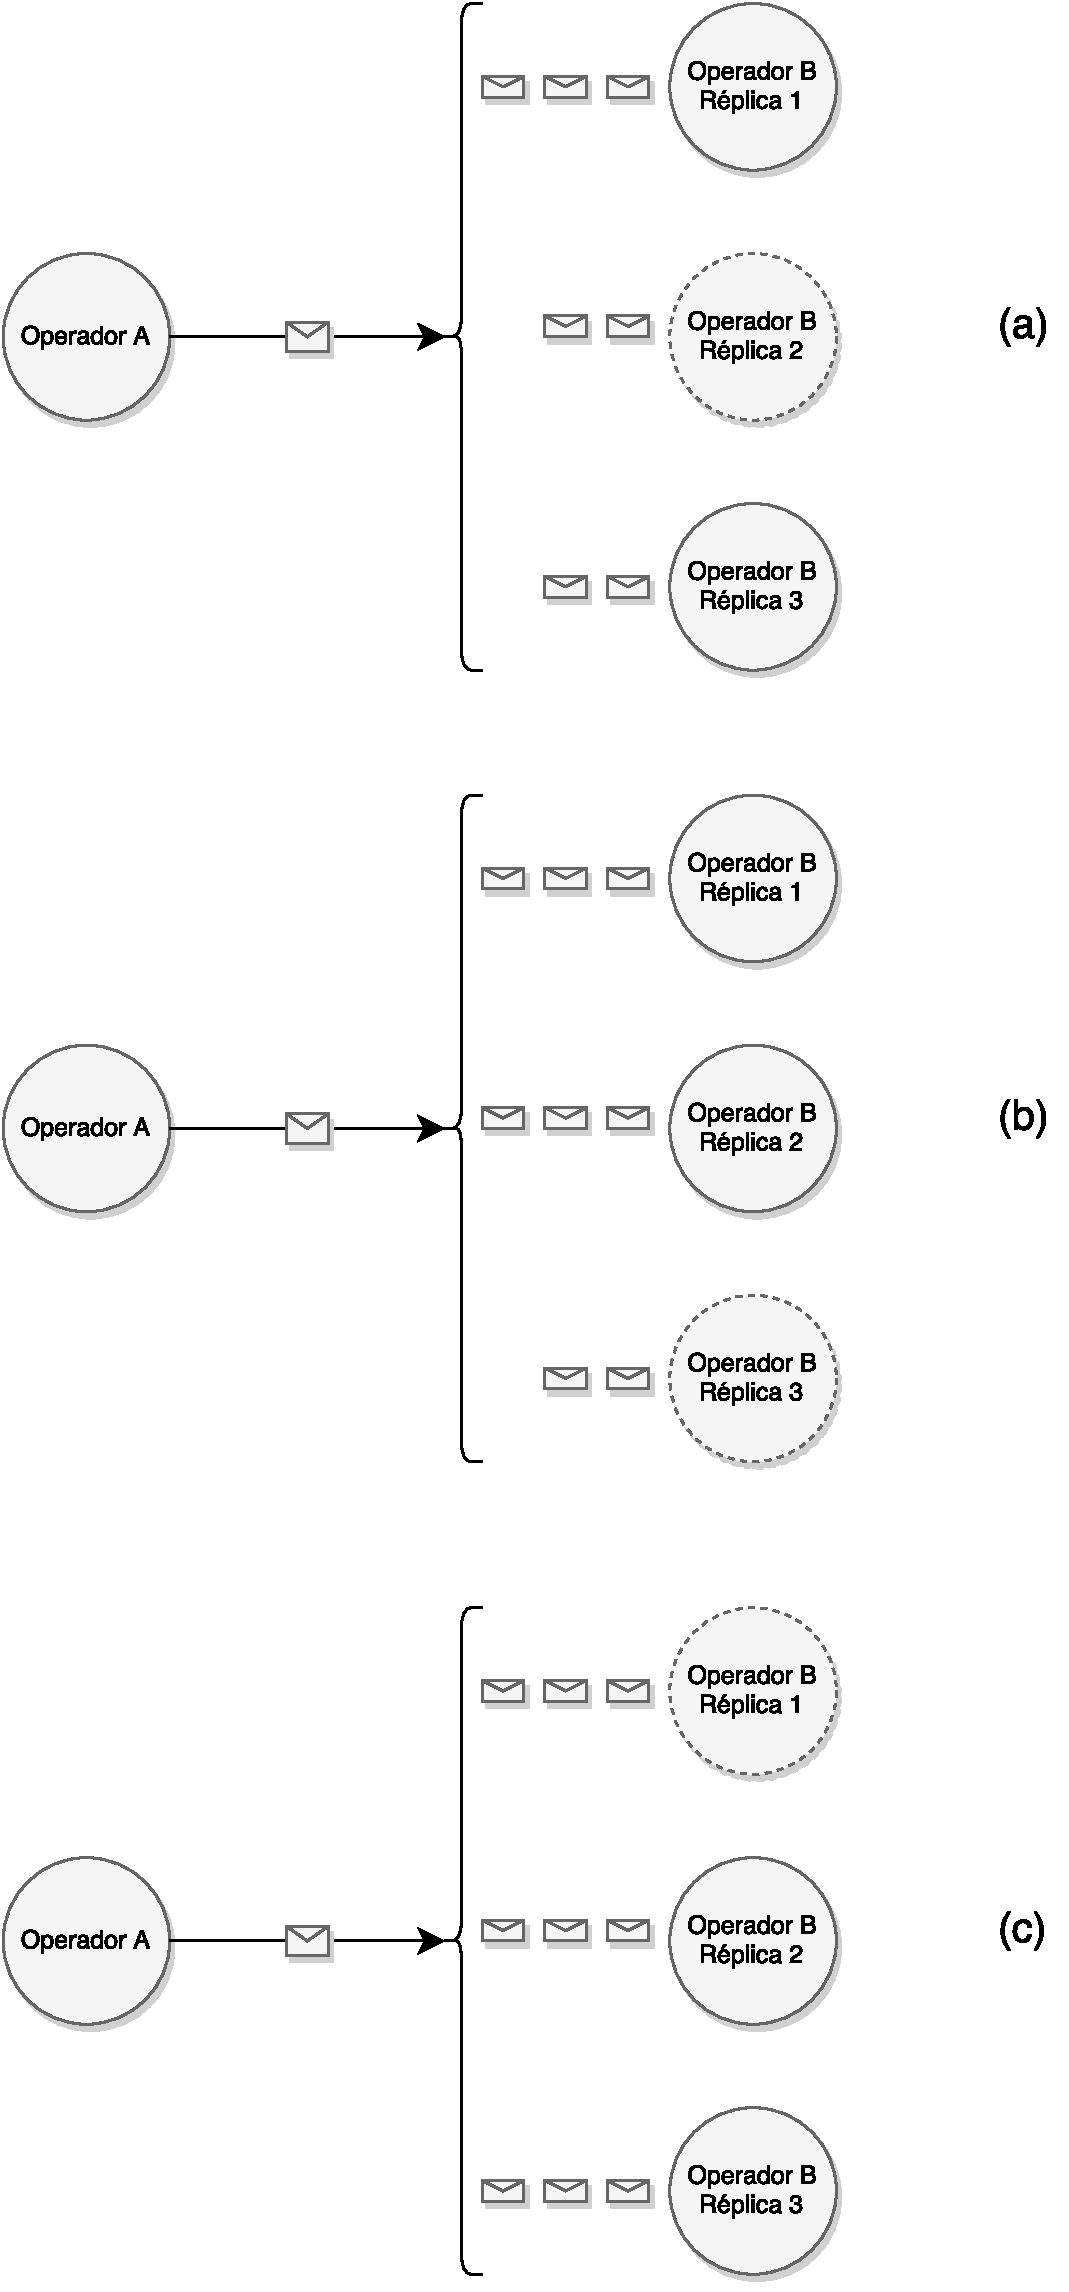
\includegraphics[scale=0.4]{images/DistribucionCarga.pdf}
	\caption[Distribuci\'on de la carga entre las r\'eplicas.]{Distribuci\'on de la carga entre las r\'eplicas.\\Fuente: Elaboraci\'on propia.}
	\label{fig:distCarga}
\end{figure}

%En el Algoritmo \ref{alg:distCarga} se describe la distribuci\'on de carga planteada anteriormente, el cual se ha implementado en S4 para ejecutar los experimentos.

%\begin{algorithm}[!ht]
%	\caption{Distribuci\'on de carga entre las r\'eplicas de un operador.}
%	\label{alg:distCarga}
%	\begin{algorithmic}[1]
%	\REQUIRE Evento $\epsilon$ y operador $\phi$.
%	\ENSURE Env\'io del evento a la r\'eplica disponible del operador $\phi$.
%	\STATE $\theta \leftarrow minTamanoCola(\phi)$ \COMMENT Se escoge la r\'eplica que posea menor cola
%	\STATE $envioEvento(\epsilon,\theta$)
%	\end{algorithmic}
%\end{algorithm}

\section{Dise\~no de los experimentos}
Para los experimentos se han dise\~nado tres aplicaciones: una que realiza operaciones con estado, otra que realiza operaciones sin estado, y otra aplicaci\'on sint\'etica. En el caso que la aplicaci\'on posea estado, significa que el operador guarda variables al procesar con el transcurso del tiempo, las cuales son entregadas cada cierto tiempo o al finalizar la ejecuci\'on del sistema. Este tipo de aplicaciones son las m\'as utilizadas, dado que utilizan contadores o variables globales, las cuales son necesarias para el an\'alisis de los datos. Un ejemplo de esto, es un sistema que cuenta las palabras de un texto y que env\'ia la cantidad de palabras contadas cada cierto tiempo. Si bien, las aplicaciones sin estado no son tan utilizadas, se consideraron importantes para la validaci\'on del modelo, dado que son las aplicaciones m\'as simples y b\'asicas de dise\~nar y ejecutar. Por otra parte, se ha generado una aplicaci\'on sint\'etica, la cual simula el procesamiento de datos por medio de la introducci\'on de retrasos de cada uno de los operadores. Cada operador es una hebra de procesamiento, para reflejar el tiempo de ejecuci\'on, por lo que se procede a dormir la hebra por un tiempo predefinido, el cual est\'a determinado por la complejidad del operador. Los operadores m\'as complejos son dormidos por una mayor cantidad de tiempo.

%Se genero una aplicacion sintetica donde se simula el procesamiento de datos por medio de la introduccion de retrasos en cada uno de los operadores. Cada operador es una hebra de procesamiento, para reflejar el tiempo de procesamiento, se procede a dormir la hebra por un tiempo predefinido determinado por la complejidad del operador. Operadores mas complejos ser\'an dormidos una mayor cantidad de tiempo. 

Para la generaci\'on del \textit{stream} de la fuente de datos para la primera y segunda aplicaci\'on, se ha utilizado un conjunto de 4.5 millones de \textit{tweets}\footnote{Un \textit{tweet} es una publicaci\'on o actualizaci\'on de estado realizada en la red social \textit{Twitter}. Como tal, un \textit{tweet} es un mensaje cuyo l\'imite de extensi\'on son 140 caracteres. Puede contener letras, n\'umeros, signos y enlaces.}, los cuales fueron recolectados entre los d\'ias 27-28 de Febrero y 1-2 de Marzo de 2010, tanto en ingl\'es, portugu\'es y espa\~nol. Estos contienen informaci\'on correspondiente a la interacci\'on entre los usuarios durante el terremoto ocurrido el 27 de Febrero en Chile.

Por otra parte, el env\'io de los datos se ha realizado de dos maneras: constante y variable. El env\'io de datos constante consiste en enviar 100 eventos por segundo durante todo el experimento. El env\'io de datos variable consiste en enviar 50 eventos por segundos el primer tercio del experimento, para luego aumentar a 100 eventos por segundo en el segundo tercio, y finalmente, disminuir a 50 eventos por segundos el \'ultimo tercio de la ejecuci\'on.

\subsection{Aplicaci\'on 1: An\'alisis de \textit{tweets} en escenarios de desastres naturales}
La primera aplicaci\'on es orientada a un escenario de desastres naturales, donde se genera un grafo que realice un filtrado de palabras, identificaci\'on del idioma y conteo de palabras. Ninguno de los operadores posee estado, por lo tanto son independientes. Para la duraci\'on de esta prueba se ha considerado un tiempo de ejecuci\'on de 70 minutos, \normalsize{cuya duraci\'on est\'a basada en el \textit{benchmark} confeccionado por} \citep{ArasuCGMMRST04}. El objetivo de esta aplicaci\'on, es comprobar que el sistema dise\~nado puede funcionar con aplicaciones sin estado, las cuales son las m\'as b\'asicas y sencillas de dise\~nar en SPS, y que tienen utilidad cuando se hacen an\'alisis directo del flujo de datos.

La aplicaci\'on consta del flujo de datos, cuyos datos son la muestra de \textit{tweets} de prueba, y cuatro operadores, los cual son denominados \textit{Stopword}, \textit{Language}, \textit{Counter} y \textit{MongoDB}.

\paragraph{Stopword:} es el operador encargado de leer el \textit{tweet} y remover las palabras que no son relevantes para el an\'alisis de \'este, usando una bolsa de palabras (\textit{stopwords}). De esta manera, se puede analizar el texto usando las palabras m\'as representativas de \'este y as\'i entregar informaci\'on m\'as precisa.

\paragraph{Language:} es el operador encargado de identificar el lenguaje existente en el \textit{tweet}, para esto se utilizado una librer\'ia \textit{Apache Tika} \citep{mattmann2011tika}. Con \'esta se puede realizar un filtro del idioma de los tweets, de tal manera que en caso de ser requerido, s\'olo contin\'uen los de un idioma en espec\'ifico, en nuestro caso el espa\~nol.

\paragraph{Counter:} es el operador encargado de contar la cantidad de palabras que existen en el \textit{tweet} seg\'un una bolsa de palabras proporcionada por el programador. Para esta prueba se ha utilizado una bolsa de 26.000 palabras en espa\~nol. Con esto se pueden detectar los \textit{tweets} que poseen mayor cantidad de palabras claves asociados a una tem\'atica o evento en particular.

\paragraph{MongoDB:} es el operador encargado de guardar en la base de datos el evento seg\'un los atributos que posee, ya sea por el \textit{tweet} original, sin \textit{stopword}, idioma y cantidad de palabras claves existentes en \'el. Para esto, se ha utilizado el motor de base de datos no relacional \textit{MongoDB} \citep{chodorow2013mongodb}.

En la Figura \ref{fig:primeraAplicacion} se muestra un ejemplo de la aplicaci\'on con sus distintos operadores y relaciones. Las flechas muestran la direcci\'on del flujo de datos emitido por la fuente y los operadores.

\begin{figure}[!hb]
	\centering
	\captionsetup{justification=centering}
		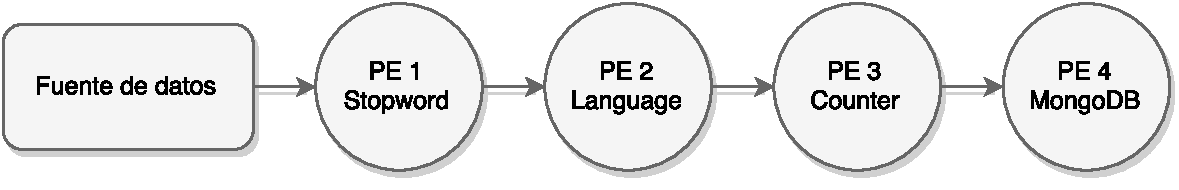
\includegraphics[scale=0.6]{images/App1.pdf}
	\caption[Aplicaci\'on 1: An\'alisis de \textit{tweets} en escenarios de desastres naturales.]{Aplicaci\'on 1: An\'alisis de \textit{tweets} en escenarios de desastres naturales.\\Fuente: Elaboraci\'on propia.}
	\label{fig:primeraAplicacion}
\end{figure}

\subsection{Aplicaci\'on 2: Contador de palabras en muestras de textos}
La segunda aplicaci\'on consiste en un contador de palabras, la cual cuenta la cantidad de veces que se repite una palabra en un conjunto de datos seg\'un una bolsa de palabras establecida por el usuario. Esta aplicaci\'on se considera con estado, debido que es necesario un contador en el operador, de tal manera de contar la cantidad de veces que se repite cierta palabra seg\'un una bolsa de palabras definida. Con esta aplicaci\'on es posible analizar posteriormente las palabras m\'as frecuentes emitidas por los usuarios de la red social seg\'un un listado de palabras claves. Para la duraci\'on de esta prueba se ha considerado un tiempo de 70 minutos, al igual que en la anterior aplicaci\'on. El objetivo de esta aplicaci\'on es validar el modelo dise\~nado con aplicaciones con estado, las cuales son las m\'as aplicadas, debido que se realizan an\'alisis generales de los datos, como el caso de los \textit{trending topics} o frecuencia de palabras.

La aplicaci\'on consta del flujo de datos, cuyos datos de entrada son la muestra de \textit{tweets} de prueba, y tres operadores, denominados \textit{Split}, \textit{Counter} y \textit{Merge}.

\paragraph{Split:} es el operador encargado de dividir el \textit{tweet}, y enviar un arreglo con las palabras que posee al operador \textit{Counter}.

\paragraph{Counter:} es el operador encargado de llevar las estad\'isticas de los contadores de cada palabra. Cuando recibe un evento, el operador aumenta el contador de las palabras que corresponde al arreglo de palabras enviado. Las estad\'isticas son enviadas cada 10 segundos al operador Merge, de tal manera de no enviar flujo constante al siguiente operador y sobrecargar al operador.

\paragraph{Merge:} es el operador encargado de unir las distintas estad\'isticas enviadas por las distintas r\'eplicas del operador Counter, sumando los valores que corresponde a las palabras enviadas.

En la Figura \ref{fig:segundaAplicacion} se muestra un ejemplo de la segunda aplicaci\'on con sus distintos operadores y sus relaciones, de igual manera que en el caso anterior, las flechas reflejan el flujo de datos. Cabe destacar que el \'unico operador que puede replicarse es el \textit{Counter}, debido que el operador \textit{Split} y \textit{Merge} son operadores que soportan la replicaci\'on del operador \textit{Counter}, como se explic\'o en las t\'ecnicas de balance de carga en la Secci\'on \ref{sec:fisionBC}.

\begin{figure}[!ht]
	\centering
	\captionsetup{justification=centering}
		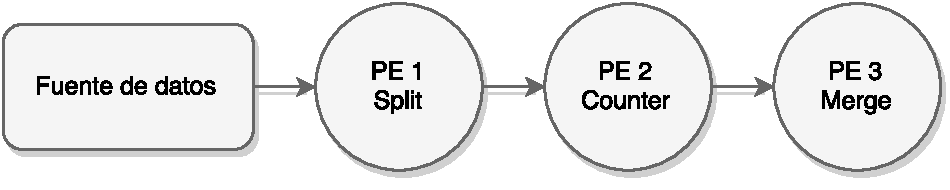
\includegraphics[scale=0.6]{images/App2.pdf}
	\caption[Aplicaci\'on 2: Contador de palabras en muestras de textos.]{Aplicaci\'on 2: Contador de palabras en muestras de textos.\\Fuente: Elaboraci\'on propia.}
	\label{fig:segundaAplicacion}
\end{figure}

\subsection{Aplicaci\'on 3: Aplicaci\'on sint\'etica}
%La tercera aplicaci\'on consta de tres operadores sint\'eticos, los cuales duermen a la hebra asignada al operador un determinado per\'iodo de tiempo, simulando el tiempo de procesamiento le toma al operador, \normalsize{cuya duraci\'on est\'a basada en el \textit{benchmark} confeccionado por} \citep{ArasuCGMMRST04}. El objetivo de este tipo de aplicaci\'on, es analizar los costos que posee el sistema implementando.

La tercera aplicaci\'on conste de tres operadores sint\'eticos, los cuales son hebras de procesamiento que llevan a cabo una tarea espec\'ifica, dependiendo del tipo de operador que representa. Para simular el procesamiento de eventos, se procede a dormir la hebra en el momento que recibe el evento por un tiempo determinado experimental de acuerdo a la complejidad del operador. Esto quiere decir, los operadores m\'as complejos toman mayor tiempo en procesar cada evento, por ende la hebra debe ser dormida un mayor tiempo para simular dicho comportamiento. El objetivo de este experimento es evaluar los costos en t\'erminos de memoria y uso de la CPU que posee el modelo el\'astico propuesto.

%La Tabla \ref{tab:app3-time} muestra el per\'iodo de tiempo que duerme cada PE \normalsize{la hebra que tiene asignada}. Los tiempos que se han considerado para esta prueba son para generar una sobrecarga en el primer y segundo operador, de tal manera que despu\'es afecten al tercer operador. Para la duraci\'on de esta prueba se ha considerado un tiempo de 15 minutos.

Para definir los tiempos de procesamientos de las hebras, se crearon operadores reales con complejidades diferentes y midiendo el tiempo que tarda en procesar un evento. Con esto tiempos promedios obtenidos, se ha definido el per\'iodo de tiempo que duerme la hebra en cada uno de los PEs, los cuales se presentan en la Tabla \ref{tab:app3-time}.

%Para definir los tiempos de procesamiento de las hebras, se crearon operadores reales con complejidades diferentes y se midio el tiempo que tomaba el procesamiento desde que un evento ingresaba al operador hasta que sal\'ia procesado. Los tiempos promedios obtenidos para los operadores analizados se presentan en la tabla 5.1

\begin{table}[!ht]
\centering
\captionsetup{justification=centering}
\caption[Per\'iodo de tiempo que duerme la hebra asignada al PE.]{Per\'iodo de tiempo que duerme la hebra asignada al PE.\\Fuente: Elaboraci\'on propia.}
\begin{tabular}{| c | c |}
\hline
PE & Tiempo (ms) \\ \hline
1 & 20 \\
2 & 30 \\
3 & 15 \\\hline
\end{tabular}
\label{tab:app3-time}
\end{table}

En la Figura \ref{fig:terceraAplicacion} se muestra un ejemplo de la tercera aplicaci\'on con sus distintos operadores y sus relaciones, de igual manera que en los casos anteriores, las flechas reflejan el flujo de datos.

\begin{figure}[!ht]
	\centering
	\captionsetup{justification=centering}
		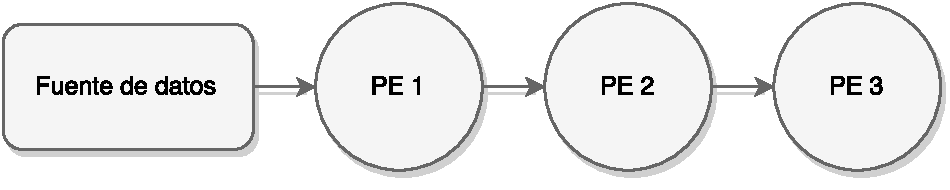
\includegraphics[scale=0.6]{images/App3.pdf}
	\caption[Aplicaci\'on 3: Aplicaci\'on sint\'etica.]{Aplicaci\'on 3: Aplicaci\'on sint\'etica.\\Fuente: Elaboraci\'on propia.}
	\label{fig:terceraAplicacion}
\end{figure}

\section{Evaluaci\'on}
Para la ejecuci\'on de los experimentos, se ha utilizado un servidor con sistema operativo Ubuntu 14.04.2 LTS, cuyo procesador es un Intel Xeon CPU E5-2650 v2 de 2.60 GHz y con 32 GB de RAM. Cabe recalcar, que el lenguaje de programaci\'on es Java, debido a la integraci\'on del sistema propuesto en el SPS utilizado. La configuraci\'on de S4 es detallada en el Anexo \ref{apendice:config-comm-S4}.

Para la ventana de tiempo del recolector de datos se utiliza un valor de $T_m = 1seg$. Para el administrador de replicas los par\'ametros del numero de replicas a crear por cada algoritmo se definieron con los valores $\omega = 1$ (reactivo), y $\theta = 5$ (predictivo). Las ventanas de tiempo entre las ejecuciones de los algoritmos son $T_r = 5seg$ y $T_p = 100seg$ respectivamente. Los par\'ametros del algoritmo predictivo para estos experimentos son una cantidad de muestras de $n = 100$, una cantidad de iteraciones para el c\'alculo de la distribuci\'on estacionaria de $\upsilon = 100000$ y una desviaci\'on est\'andar de $\alpha = 0.25$ entre las variables aleatorias obtenidas por la distribuci\'on estacionaria. La cantidad de alertas consecutivas para activar el an\'alisis del algoritmo reactivo es de $\beta = 2$.

\subsection{Aplicaci\'on 1: An\'alisis de \textit{tweets} en escenarios de desastres naturales}
Con la primera aplicaci\'on se efectuaron dos experimentos, donde el primero consta de un env\'io constante de eventos, y el segundo de un env\'io variable. En ambos experimentos, se han considerado dos pruebas, la primera consiste en la ejecuci\'on de la aplicaci\'on en un sistema SPS con el uso del modelo el\'astico, y la segunda sin el uso de \'este.

%Para el an\'alisis de los experimentos, se ha considerado la cantidad promdio de eventos procesados en un per\'iodo, la cantidad total de eventos procesados y las estad\'isticas de cada PE en el transcurso de la ejecuci\'on de la aplicaci\'on.

Para el an\'alisis de los experimentos, se ha considerado \normalsize{el rendimiento y la cantidad de r\'eplicas del grafo} y la cantidad total de eventos procesados. \normalsize{En el Anexo} \ref{apendice:estadisticas-operadores} \normalsize{se presentan las estad\'isticas de cada uno de los operadores.}

%%% EXP1-CONSTANTE OPERADORES %%%

%Las Figuras \ref{fig:app1-uniform-statusStopwordPE-cm} y \ref{fig:app1-uniform-statusStopwordPE-sm} corresponden al primer experimento y muestran las estad\'isticas del primer operador del grafo, con y sin uso del modelo en la carga de los operadores, respectivamente, ambas con un env\'io constante de eventos desde la fuente de datos. Se puede observar en el primer gr\'afico una tasa de llegada ($\lambda$) constante, a diferencia del segundo gr\'afico, donde varia a partir del segundo 2600.

%El cambio de la tasa de llegada del segundo gr\'afico se debe a la sobrecarga que existe en el operador, debido que no puede procesar todos los eventos que son enviados a \'este, por lo que es un sistema inestable, es decir, $\rho > 1$. Esto genera una acumulaci\'on de eventos en el \textit{buffer} del operador, de tal manera que al llenarse, bloquea la recepci\'on de eventos. Por lo que se debe esperar que se liberen eventos del \textit{buffer}, pero como la tasa de rendimiento es baja, al desencolarse, inmediatamente llegada otro evento que vuelve a llenarlo, por lo que la cola se mantiene constante despu\'es del segundo 2600. Es por esto mismo que la tasa de llegada disminuye aproximadamente al mismo valor de la tasa de procesamiento.

%Por otra parte, la tasa de rendimiento ($\rho$) graficada en la Figura \ref{fig:app1-uniform-statusStopwordPE-cm} se estabiliza dentro de los primeros 100 segundos, debido que el modelo el\'astico detecta el operador sobrecargado y lo replica. A diferencia de la Figura \ref{fig:app1-uniform-statusStopwordPE-sm}, en el cual el operador posee una tasa de rendimiento inestable que fluct\'ua entre 1 y 2, hasta el segundo 2600, donde disminuye debido que la tasa de llegada es menor. Cabe destacar que este operador posee un alto costo computacional, debido que existe una gran cantidad de palabras que debe analizar para cada una de las palabras del \textit{tweet}, por lo que es necesario crear otra r\'eplica.

%En las Figuras \ref{fig:app1-uniform-statusLanguagePE-cm} y \ref{fig:app1-uniform-statusLanguagePE-sm} se observa el siguiente operador de la topolog\'ia del grafo, el cual no presenta sobrecarga, a excepci\'on del segundo 2400, donde en el caso sin uso del modelo disminuye considerablemente la tasa de procesamiento del PE. Si analizamos las Figuras \ref{fig:app1-uniform-statusStopwordPE-sm} y \ref{fig:app1-uniform-statusLanguagePE-sm}, empiezan aproximadamente desde el rango de tiempo (2400s, 2600s) los problemas de procesamiento de los operadores, por lo tanto, se puede deducir que si el problema surge en un operador no es un problema aislado, sino que tambi\'en influye a los siguientes operadores.

%Se puede observar como con el transcurso de los primeros 100 segundos en la Figura \ref{fig:app1-uniform-statusCounterPE-cm}, aumenta la cantidad de r\'eplicas hasta llegar a 5, el cual es su \'optimo, para ir procesando la cantidad de eventos actuales y disminuir la cola existente en el sistema. Esto en contraposici\'on a la Figura \ref{fig:app1-uniform-statusCounterPE-sm}, donde la inexistencia de replicaci\'on, genera una cola la cual se mantiene constante en el segundo 2400.

%Finalmente, se encuentra el \'ultimo operador, el cual no presenta grandes problemas de procesamiento tanto en las Figuras \ref{fig:app1-uniform-statusMongoPE-cm} y \ref{fig:app1-uniform-statusMongoPE-sm}. Esto se debe a que el tiempo de procesamiento es bajo y nunca llega una cantidad de eventos considerable para provocar una sobrecarga. Adem\'as, es importante destacar que en la Figura \ref{fig:app1-uniform-statusMongoPE-sm} se registra una menor tasa de llegada, con un promedio de $83\%$ menos de eventos que un SPS ejecutado con el modelo el\'astico.

%\begin{figure}[p]
%\centering
%    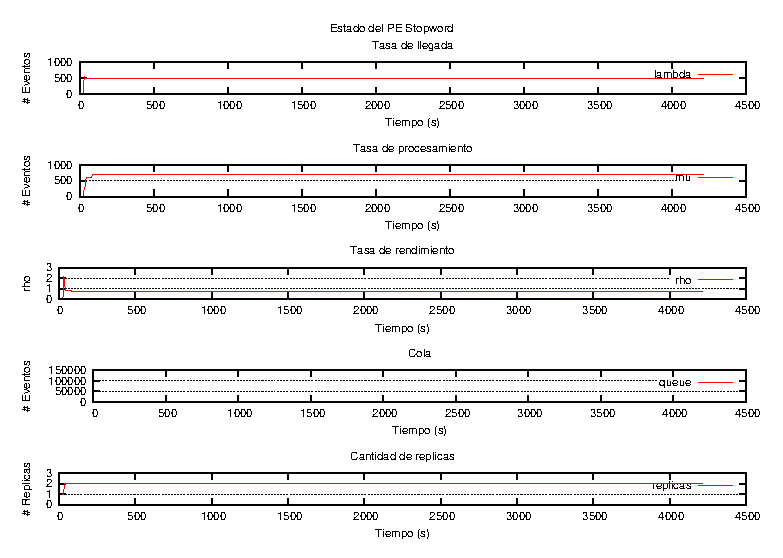
\includegraphics[scale=1.1]{images/exp/app1/uniform/cm/statusStopwordPE.eps}
%    \caption{Estad\'isticas del PE Stopword en la primera aplicaci\'on con un env\'io constante de la fuente de datos con uso del modelo.}
%    \label{fig:app1-uniform-statusStopwordPE-cm}
%\end{figure}
%
%\begin{figure}[p]
%\centering
%    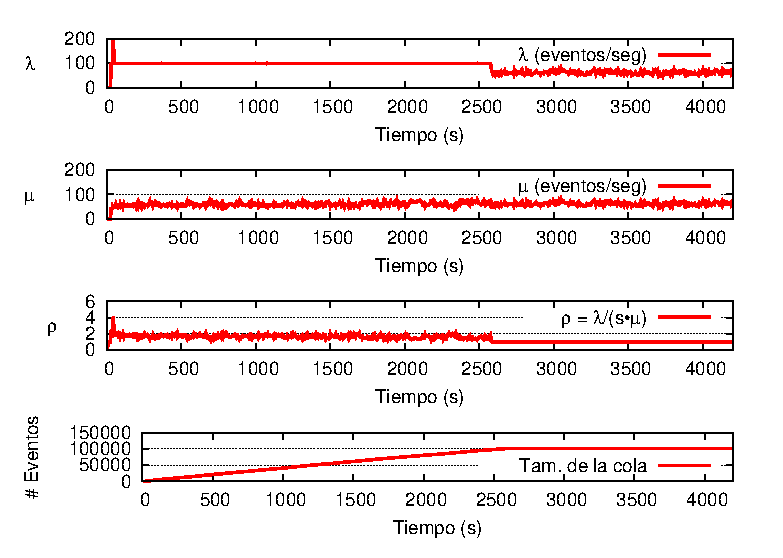
\includegraphics[scale=1.1]{images/exp/app1/uniform/sm/statusStopwordPE.eps}
%    \caption{Estad\'isticas del PE Stopword en la primera aplicaci\'on con un env\'io constante de la fuente de datos sin uso del modelo.}
%    \label{fig:app1-uniform-statusStopwordPE-sm}
%\end{figure}
%
%\begin{figure}[p]
%\centering
%    \includegraphics[scale=1.1]{images/exp/app1/uniform/cm/statusLanguagePE.eps}
%    \caption{Estad\'isticas del PE Language en la primera aplicaci\'on con un env\'io constante de la fuente de datos con uso del modelo.}
%    \label{fig:app1-uniform-statusLanguagePE-cm}
%\end{figure}
%
%\begin{figure}[p]
%\centering
%    \includegraphics[scale=1.1]{images/exp/app1/uniform/sm/statusLanguagePE.eps}
%    \caption{Estad\'isticas del PE Language en la primera aplicaci\'on con un env\'io constante de la fuente de datos sin uso del modelo.}
%    \label{fig:app1-uniform-statusLanguagePE-sm}
%\end{figure}
%
%\begin{figure}[p]
%\centering
%    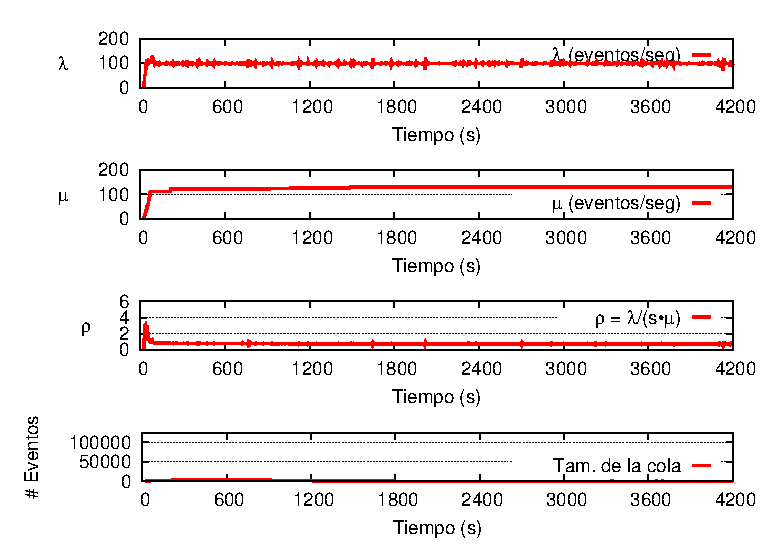
\includegraphics[scale=1.1]{images/exp/app1/uniform/cm/statusCounterPE.eps}
%    \caption{Estad\'isticas del PE Counter en la primera aplicaci\'on con un env\'io constante de la fuente de datos con uso del modelo.}
%    \label{fig:app1-uniform-statusCounterPE-cm}
%\end{figure}
%
%\begin{figure}[p]
%\centering
%    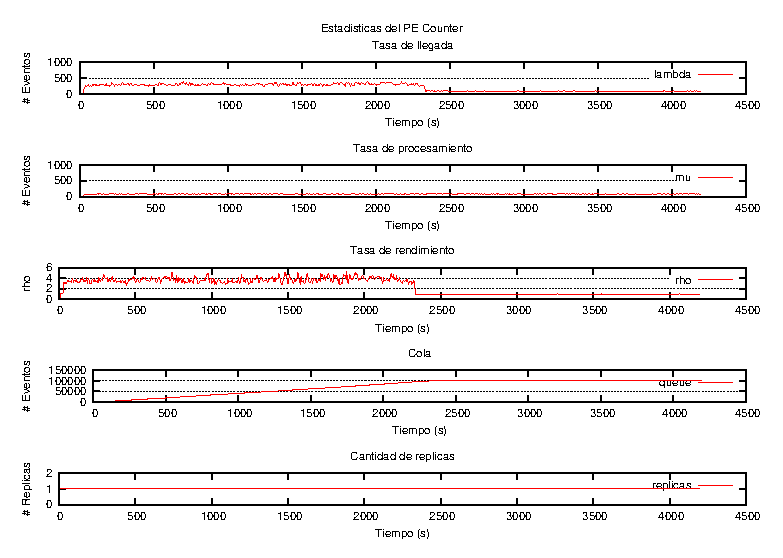
\includegraphics[scale=1.1]{images/exp/app1/uniform/sm/statusCounterPE.eps}
%    \caption{Estad\'isticas del PE Counter en la primera aplicaci\'on con un env\'io constante de la fuente de datos sin uso del modelo.}
%    \label{fig:app1-uniform-statusCounterPE-sm}
%\end{figure}
%
%\begin{figure}[p]
%\centering
%    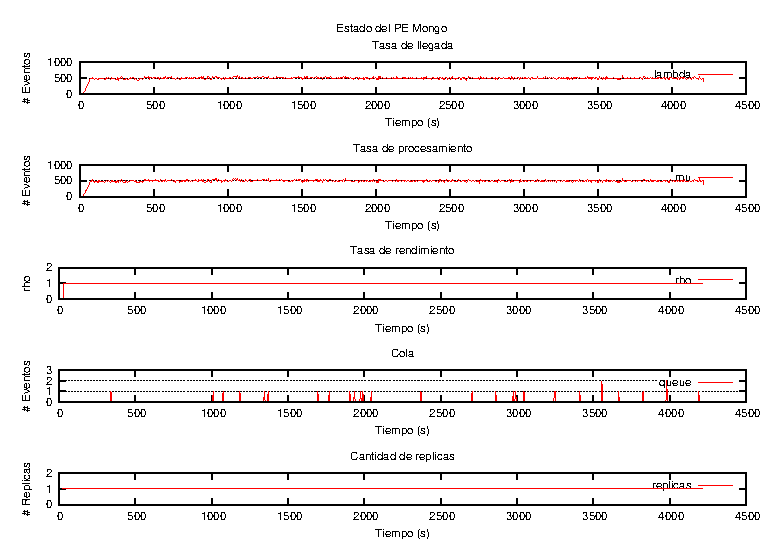
\includegraphics[scale=1.1]{images/exp/app1/uniform/cm/statusMongoPE.eps}
%    \caption{Estad\'isticas del PE Mongo en la primera aplicaci\'on con un env\'io constante de la fuente de datos con uso del modelo.}
%    \label{fig:app1-uniform-statusMongoPE-cm}
%\end{figure}
%
%\begin{figure}[p]
%\centering
%    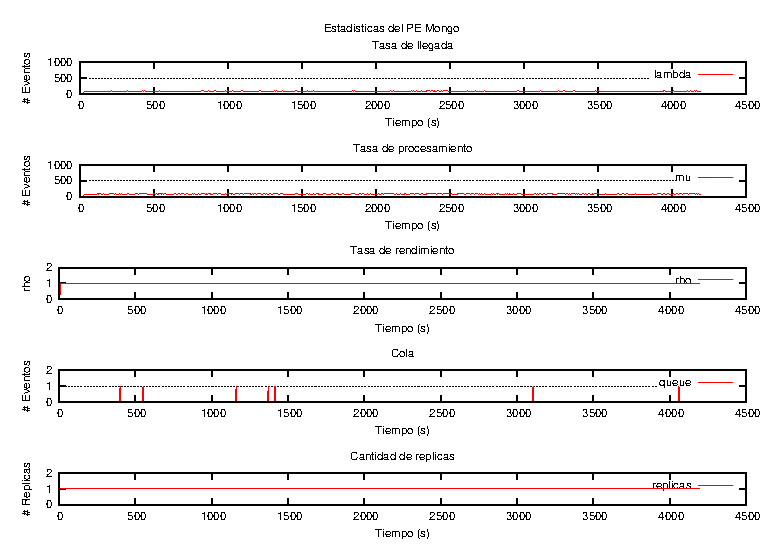
\includegraphics[scale=1.1]{images/exp/app1/uniform/sm/statusMongoPE.eps}
%    \caption{Estad\'isticas del PE Mongo en la primera aplicaci\'on con un env\'io constante de la fuente de datos sin uso del modelo.}
%    \label{fig:app1-uniform-statusMongoPE-sm}
%\end{figure}

%%% EXP1-CONSTANTE PERFORMANCE %%%

Las Figuras \ref{fig:app1-uniform-processSystem-cm} y \ref{fig:app1-uniform-processSystem-sm} \normalsize{corresponden al primer experimento y muestra el rendimiento que posee el sistema, y como var\'ia la cantidad de r\'eplicas totales del grafo seg\'un el flujo constante de datos.} En la Figura \ref{fig:app1-uniform-processSystem-cm} \normalsize{se observa que en los primero segundos existe una sobrecarga en el grafo, espec\'ificamente en los PE Stopword y Counter, por lo que el modelo detecta esta inestabilidad en el sistema y aumenta la cantidad de r\'eplicas de los operadores} (v\'ease Anexo \ref{apendice:estadisticas-operadores}), \normalsize{logrando un procesamiento promedio de  98 eventos por segundo.} En el caso de la Figura \ref{fig:app1-uniform-processSystem-sm} \normalsize{no existe un aumento en la cantidad de r\'eplicas, por lo tanto, no existe un aumento de la cantidad de datos procesados, alcanzando un promedio de 16 eventos procesados por segundo. Se puede observar que en esta figura en el segundo 2600 la tasa de entrada disminuye considerablemente, esto es resultado de la sobrecarga del sistema. Comparando ambos escenarios se puede observar que la utilizaci\'on del modelo el\'astico para esta aplicaci\'on ha logrado mejorar el rendimiento del sistema, logrando incrementar 5 veces el numero total de eventos procesados.}

\begin{figure}[!ht]
	\centering
	\captionsetup{justification=centering}
	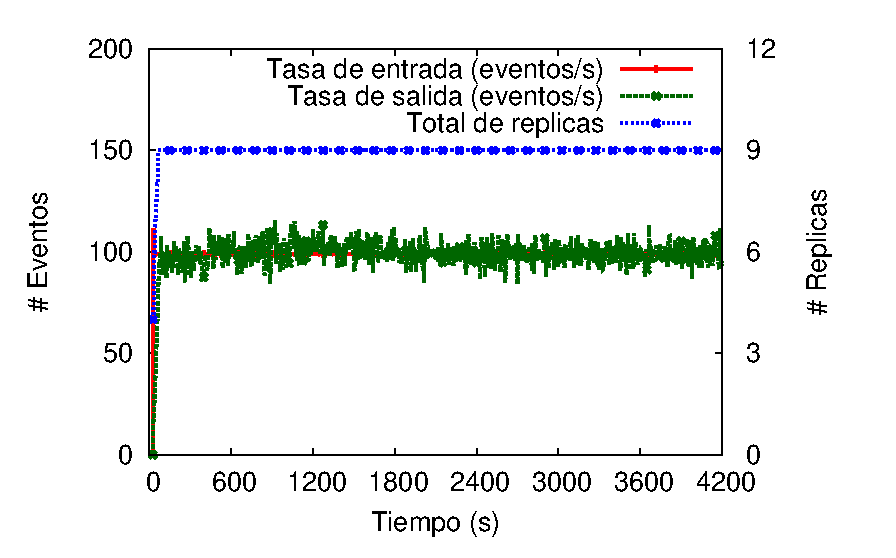
\includegraphics[scale=0.65]{images/exp/app1/uniform/cm/processSystem.eps}
    \caption[Rendimiento y cantidad de r\'eplicas totales del grafo en la primera aplicaci\'on con env\'io constante de la fuente de datos con uso del modelo.]{Rendimiento y cantidad de r\'eplicas totales del grafo en la primera aplicaci\'on con env\'io constante de la fuente de datos con uso del modelo.\\Fuente: Elaboraci\'on propia.}
	\label{fig:app1-uniform-processSystem-cm}
\end{figure}

\begin{figure}[!ht]
	\centering
	\captionsetup{justification=centering}
	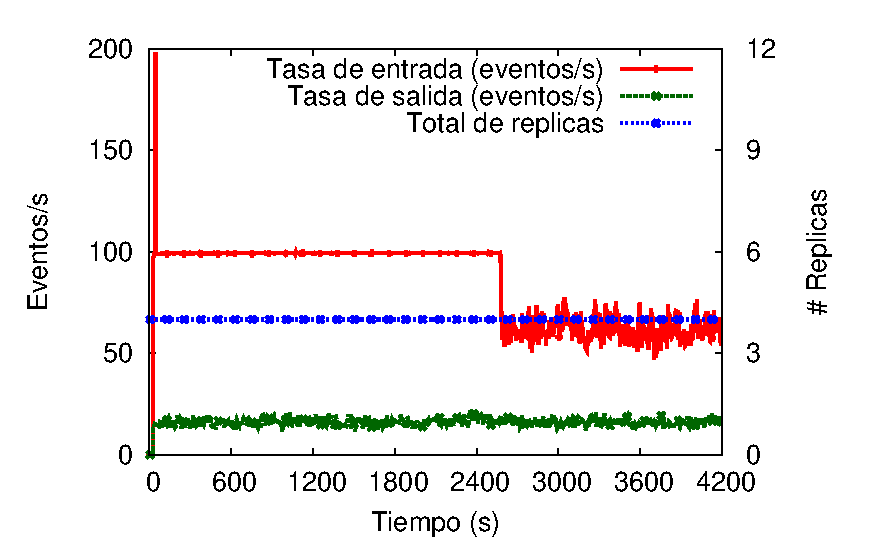
\includegraphics[scale=0.65]{images/exp/app1/uniform/sm/processSystem.eps}
    \caption[Rendimiento y cantidad de r\'eplicas totales del grafo en la primera aplicaci\'on con env\'io constante de la fuente de datos sin uso del modelo.]{Rendimiento y cantidad de r\'eplicas totales del grafo en la primera aplicaci\'on con env\'io constante de la fuente de datos sin uso del modelo.\\Fuente: Elaboraci\'on propia.}
	\label{fig:app1-uniform-processSystem-sm}
\end{figure}

%%% EXP1-CONSTANTE CANT. PROMEDIO EVENTOS PROCESADOS %%%

% Por otra parte, tambi\'en se ha analizado la cantidad promedio de eventos procesados en cada per\'iodo la cual es presentada en las Figuras \ref{fig:app1-uniform-cm-avgEventProcess} y \ref{fig:app1-uniform-sm-avgEventProcess}. Como se puede apreciar en el primero gr\'afico, en los primeros 50 segundos se observa una mejora considerable en la cantidad de eventos procesados, donde posteriormente se procesan aproximadamente 480 eventos por per\'iodo en el sistema con modelo, a diferencia del SPS sin uso del modelo, que procesa 90 eventos por per\'iodo aproximadamente, alcanzando a procesar 5 veces m\'as eventos con el modelo. Esta mejora se debe a la replicaci\'on de los operadores que poseen mayor sobrecarga, por lo que al aumentar la cantidad de r\'eplicas, aumenta la tasa de procesamiento, lo que significa mayor cantidad de flujo para el pr\'oximo operador.

%\begin{figure}[ht]
%\centering
%
%\begin{minipage}[c]{0.45\textwidth}
%\centering
%    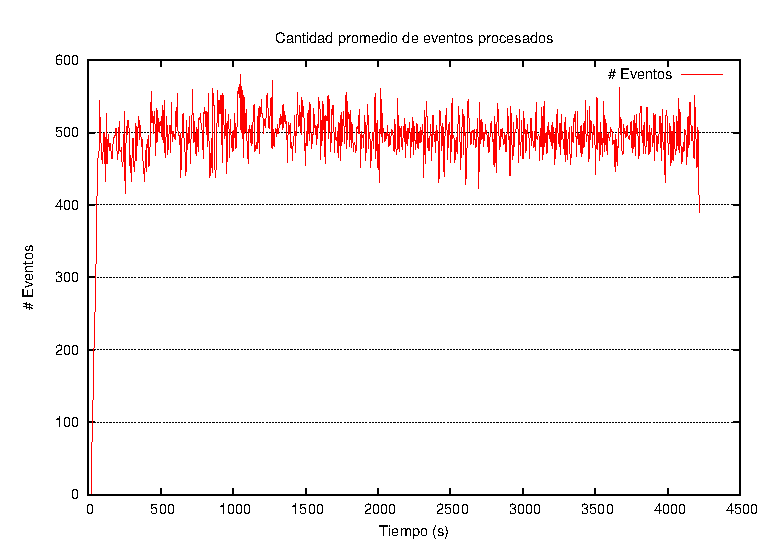
\includegraphics[width=\textwidth]{images/exp/app1/uniform/cm/avgEventProcess.eps}
%    \caption{Cantidad promedio de eventos procesados en cada per\'iodo en la primera aplicaci\'on con un env\'io constante de la fuente de datos con uso del modelo.}
%    \label{fig:app1-uniform-cm-avgEventProcess}
%\end{minipage} \hspace*{1cm}
%\begin{minipage}[c]{0.45\textwidth}
%\centering
%    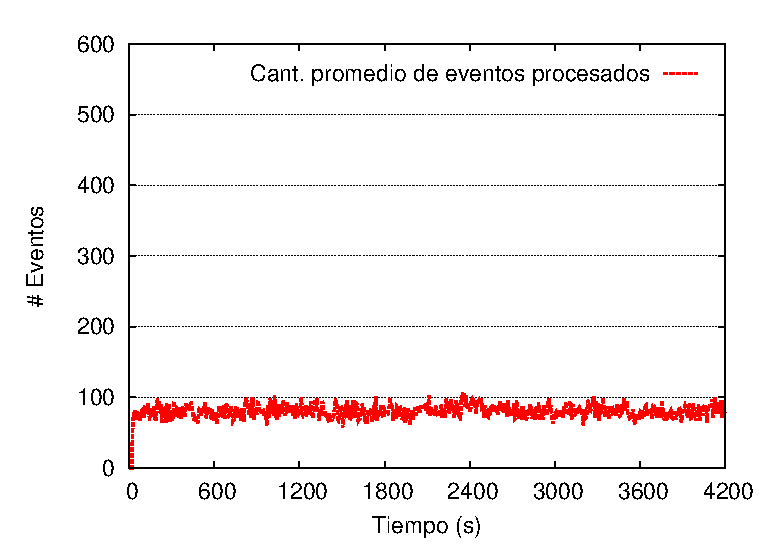
\includegraphics[width=\textwidth]{images/exp/app1/uniform/sm/avgEventProcess.eps}
%    \caption{Cantidad promedio de eventos procesados en cada per\'iodo en la primera aplicaci\'on con un env\'io constante de la fuente de datos sin uso del modelo.}
%    \label{fig:app1-uniform-sm-avgEventProcess}
%\end{minipage}
%
%\end{figure}

%%% EXP1-CONSTANTE EVENTOS TOTALES PROCESADOS %%%
En las Figuras \ref{fig:app1-uniform-eventCount-cm} y \ref{fig:app1-uniform-eventCount-sm} se presenta la cantidad total de eventos procesados en el transcurso de la ejecuci\'on en cada uno de los operadores, con y sin uso del modelo respectivamente. En el primer gr\'afico los cuatro operadores del SPS van aumentando la cantidad total de eventos procesados linealmente y con la misma pendiente, tan s\'olo existe una menor cantidad de eventos procesados en el tercer PE, lo cual se traslada al cuarto PE, debido a que al procesar menor cantidad de eventos en el tercer PE, llega una menor cantidad de eventos al cuarto PE. En este gr\'afico se alcanza un total de 401.618 eventos procesados. En cambio, en el segundo gr\'afico las curvas de cantidad de eventos procesados son muy distintas entre los distintos operadores, lo cual se ve reflejado desde la cantidad de eventos procesados en el primer operador hasta la cantidad total de eventos procesados por el sistema, el que alcanza un total de 67.141 eventos. Por lo que con el uso del modelo el\'astico se ha procesado 6 veces m\'as eventos que los procesados durante el mismo per\'iodo de tiempo sin el uso de \'este.

\begin{figure}[!ht]
	\centering
	\captionsetup{justification=centering}
    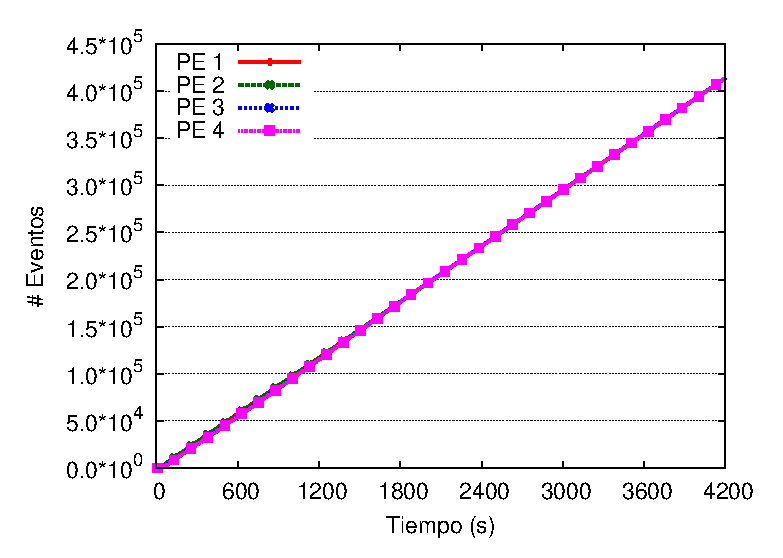
\includegraphics[scale=0.7]{images/exp/app1/uniform/cm/eventCount.eps}
    \caption[Cantidad total de eventos procesados en la primera aplicaci\'on con un env\'io constante de la fuente de datos con uso del modelo.]{Cantidad total de eventos procesados en la primera aplicaci\'on con un env\'io constante de la fuente de datos con uso del modelo.\\Fuente: Elaboraci\'on propia.}
    \label{fig:app1-uniform-eventCount-cm}
\end{figure}

\begin{figure}[!ht]
	\centering
	\captionsetup{justification=centering}
    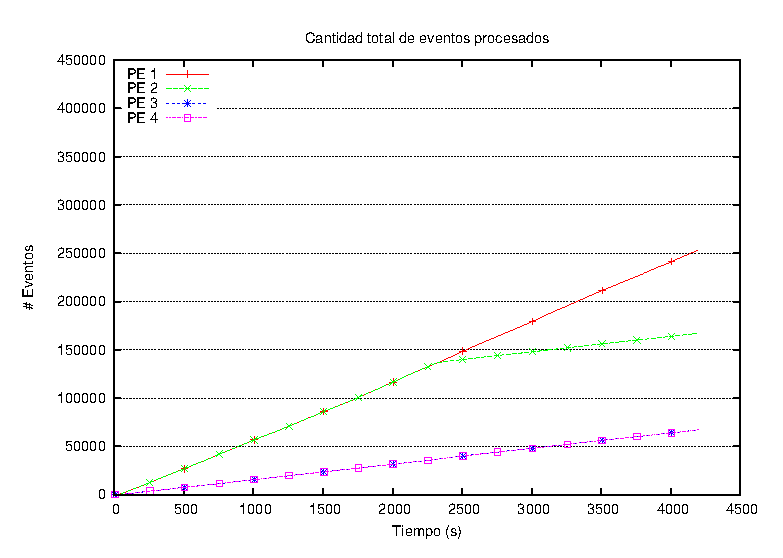
\includegraphics[scale=0.7]{images/exp/app1/uniform/sm/eventCount.eps}
    \caption[Cantidad total de eventos procesados en la primera aplicaci\'on con un env\'io constante de la fuente de datos sin uso del modelo.]{Cantidad total de eventos procesados en la primera aplicaci\'on con un env\'io constante de la fuente de datos sin uso del modelo.\\Fuente: Elaboraci\'on propia.}
    \label{fig:app1-uniform-eventCount-sm}
\end{figure}

%%% EXP1-VARIABLE OPERADORES %%%

%En el segundo experimento se observa que en las Figuras \ref{fig:app1-normal-statusStopwordPE-cm} y \ref{fig:app1-normal-statusStopwordPE-sm}, se muestra el comportamiento del primer operador con un env\'io variable de la fuente de datos. En las estad\'isticas se aprecia que existe un comportamiento estable hasta el segundo 1100, con y sin uso del modelo. Esto se debe a que el operador no posee gran cantidad de demanda dada la tasa de llegada, la cual var\'ia en el segundo 1100, debido al aumento de la cantidad de eventos entrantes. Esto implica que el operador debe procesar mayor cantidad de datos, aumentando as\'i la cantidad de r\'eplicas del mismo. Luego en el segundo 3200 disminuye la tasa de llegada, por lo que la tasa de rendimiento vuelve a ser estable en el sistema con y sin modelo, ya que es menor la cantidad de eventos que deben ser procesados, lo que significa tambi\'en la disminuci\'on de una r\'eplica en el sistema con uso del modelo.
%
%El comportamiento variable del flujo de entrada s\'olo se puede apreciar con mayor detalle en el primer operador cuando no se usa el modelo, debido que la tasa de llegada del segundo depende de la tasa de procesamiento del primero, y como no existe un aumento de la tasa de procesamiento, s\'olo aumenta hasta lo que puede procesar con un s\'olo operador.
%
%En las Figuras \ref{fig:app1-normal-statusLanguagePE-cm} y \ref{fig:app1-normal-statusLanguagePE-sm} se observa la diferencia entre las tasas de llegada, debido a que en el primer gr\'afico, existe una variaci\'on de la tasa de llegada, dado el uso del modelo el\'astico. Esto se debe a que el primer operador no procesa todos los eventos entrantes, e implica que la tasa de llegada es constante en el segundo operador. Independiente del uso o no del modelo, no existe una sobrecarga en el operador, por lo que el comportamiento del operador siempre es estable.
%
%Luego, en las Figuras \ref{fig:app1-normal-statusCounterPE-cm} y \ref{fig:app1-normal-statusCounterPE-sm} se presenta el tercer operador, en el cual existe una sobrecarga desde el inicio del sistema. Esto se debe a la gran cantidad de palabras que debe comparar, por lo que al realizar la iteraci\'on para verificar si existe o no una palabra, requiere un alto costo computacional. En el primer gr\'afico se puede analizar que en los primeros 100 segundos, el operador aumenta a trusandoes r\'eplicas, estabiliz\'andose el rendimiento del mismo. En cambio, en el sistema sin el uso del modelo el\'astico existe una tasa de procesamiento constante, por lo que la tasa de rendimiento es inestable en el transcurso de todo el experimento. Tambi\'en se muestra una disminuci\'on en la cantidad de r\'eplicas en el segundo 3200, y esto se debe a que la cantidad de r\'eplicas necesarias para el sistema es menor, dado que el env\'io de datos de la fuente de datos ha disminuido, y por ende la tasa de llegada del PE tambi\'en.
%
%Dentro de los an\'alisis importantes que se pueden realizar al gr\'afico de la Figura \ref{fig:app1-normal-statusCounterPE-cm}, es que en el primer tercio de la prueba con uso del modelo, la cantidad \'optima de operadores fue 4, pero en el \'ultimo tercio fue de 5, siendo que ambos poseen la misma tasa de llegada. Esto se debe a que al existir 7 r\'eplicas en el segundo tercio y disminuir la tasa de llegada, se detectaron operadores ociosos. Dado que el $\rho$ del operador es menor a 0.5, por lo tanto para encontrarse a un estado estable, es necesario converger a 0.5, por lo que al estabilizarse el operador, su $\rho$ tiende a estar m\'as cerca de 0.5 que de 1. De esta manera, las tasas de rendimiento son distintas en el primer y \'ultimo tercio, por lo que puede darse que las r\'eplicas del primer tercio sea mayor que el \'ultimo tercio.
%
%Por \'ultimo, en el cuarto operador se puede apreciar en las Figuras \ref{fig:app1-normal-statusMongoPE-cm} y \ref{fig:app1-normal-statusMongoPE-sm} su comportamiento con y sin uso del modelo el\'astico respectivamente. En ambos casos se muestra una tasa de rendimiento estable, la diferencia est\'a en la tasa de llegada que posee cada uno de los sistemas, donde en el primer gr\'afico la tasa de llegada es variable, y en el segundo es constante, por lo que existe una menor tasa de rendimiento, lo que significa una menor cantidad de eventos procesados.

%\begin{figure}[p]
%\centering
%    \includegraphics[scale=1.1]{images/exp/app1/normal/cm/statusStopwordPE.eps}
%    \caption{Estad\'isticas del PE Stopword en la primera aplicaci\'on con un env\'io variable de la fuente de datos con uso del modelo.}
%    \label{fig:app1-normal-statusStopwordPE-cm}
%\end{figure}
%
%\begin{figure}[p]
%\centering
%    \includegraphics[scale=1.1]{images/exp/app1/normal/sm/statusStopwordPE.eps}
%    \caption{Estad\'isticas del PE Stopword en la primera aplicaci\'on con un env\'io variable de la fuente de datos sin uso del modelo.}
%    \label{fig:app1-normal-statusStopwordPE-sm}
%\end{figure}
%
%\begin{figure}[p]
%\centering
%    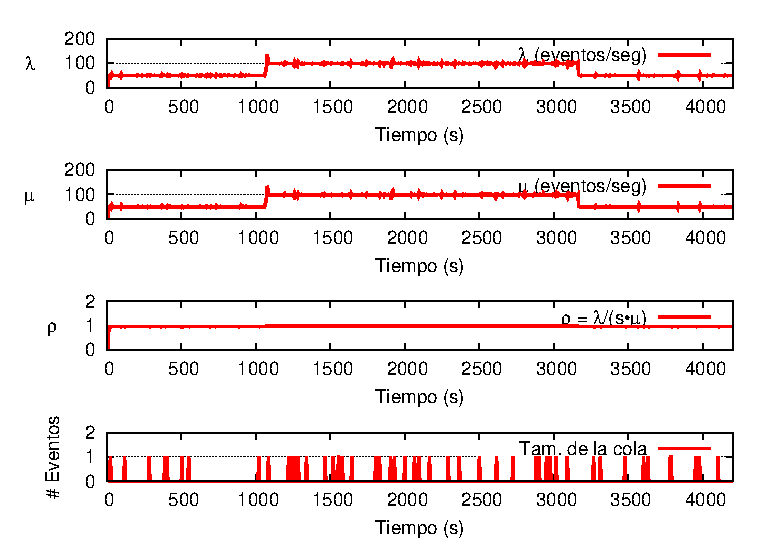
\includegraphics[scale=1.1]{images/exp/app1/normal/cm/statusLanguagePE.eps}
%    \caption{Estad\'isticas del PE Language en la primera aplicaci\'on con un env\'io variable de la fuente de datos con uso del modelo.}
%    \label{fig:app1-normal-statusLanguagePE-cm}
%\end{figure}
%
%\begin{figure}[p]
%\centering
%    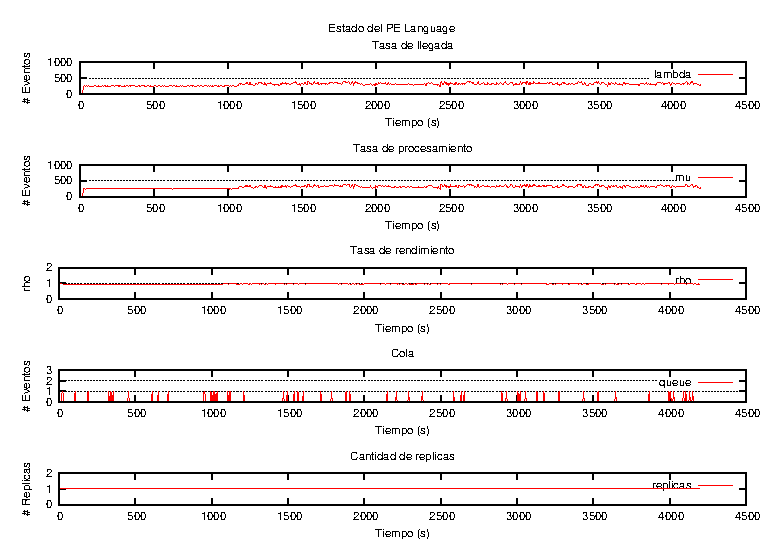
\includegraphics[scale=1.1]{images/exp/app1/normal/sm/statusLanguagePE.eps}
%    \caption{Estad\'isticas del PE Language en la primera aplicaci\'on con un env\'io variable de la fuente de datos sin uso del modelo.}
%    \label{fig:app1-normal-statusLanguagePE-sm}
%\end{figure}
%
%\begin{figure}[p]
%\centering
%    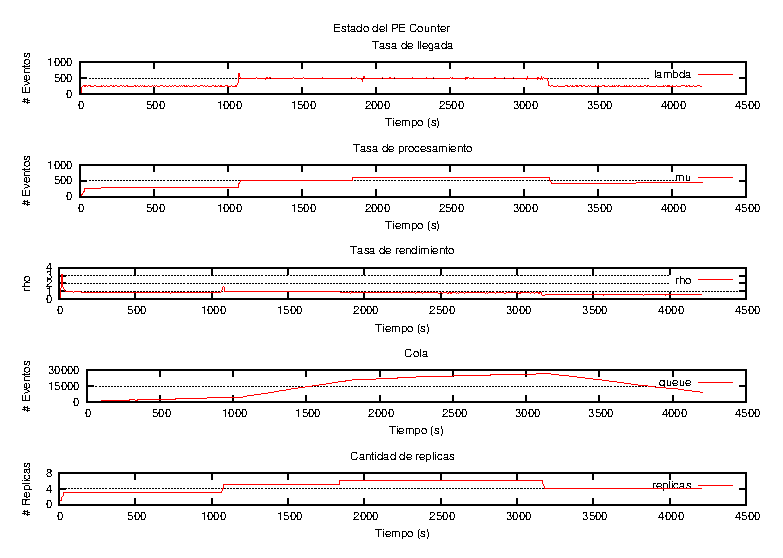
\includegraphics[scale=1.1]{images/exp/app1/normal/cm/statusCounterPE.eps}
%    \caption{Estad\'isticas del PE Counter en la primera aplicaci\'on con un env\'io variable de la fuente de datos con uso del modelo.}
%    \label{fig:app1-normal-statusCounterPE-cm}
%\end{figure}
%
%\begin{figure}[p]
%\centering
%    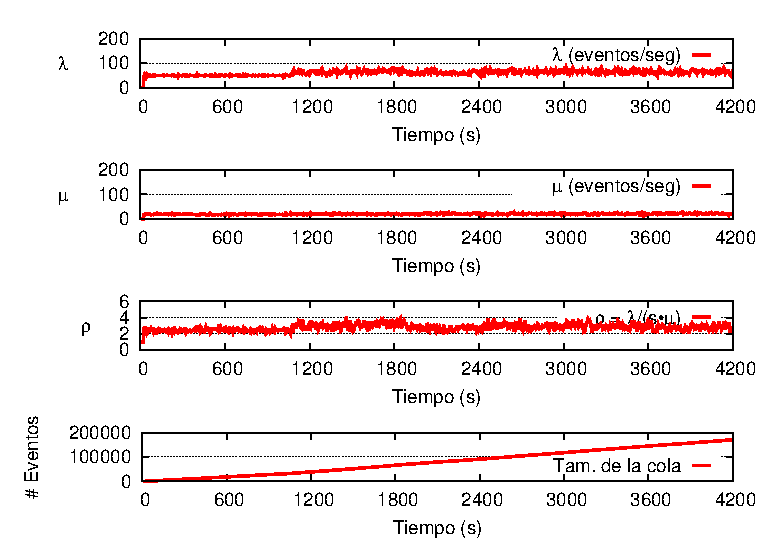
\includegraphics[scale=1.1]{images/exp/app1/normal/sm/statusCounterPE.eps}
%    \caption{Estad\'isticas del PE Counter en la primera aplicaci\'on con un env\'io variable de la fuente de datos sin uso del modelo.}
%    \label{fig:app1-normal-statusCounterPE-sm}
%\end{figure}
%
%\begin{figure}[p]
%\centering
%    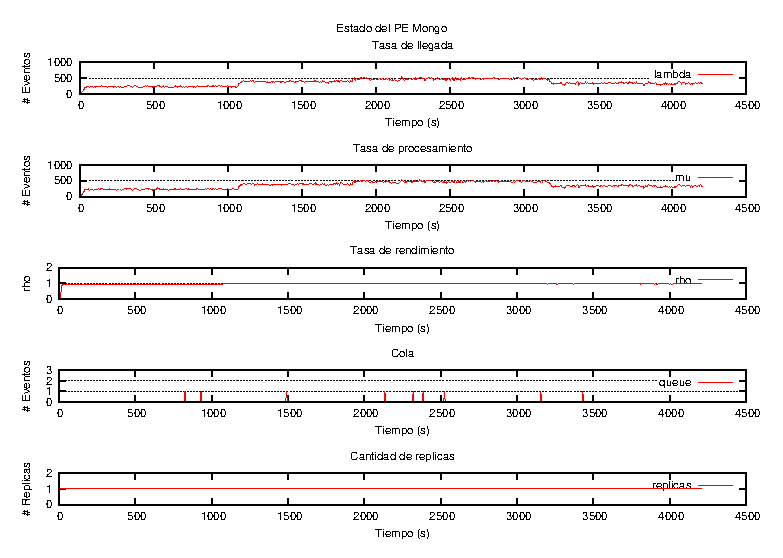
\includegraphics[scale=1.1]{images/exp/app1/normal/cm/statusMongoPE.eps}
%    \caption{Estad\'isticas del PE Mongo en la primera aplicaci\'on con un env\'io variable de la fuente de datos con uso del modelo.}
%    \label{fig:app1-normal-statusMongoPE-cm}
%\end{figure}
%
%\begin{figure}[p]
%\centering
%    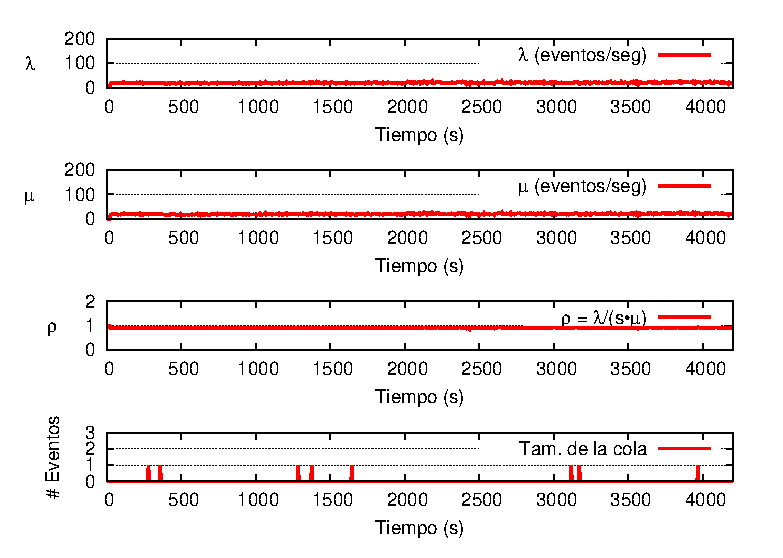
\includegraphics[scale=1.1]{images/exp/app1/normal/sm/statusMongoPE.eps}
%    \caption{Estad\'isticas del PE Mongo en la primera aplicaci\'on con un env\'io variable de la fuente de datos sin uso del modelo.}
%    \label{fig:app1-normal-statusMongoPE-sm}
%\end{figure}

%%% EXP1-VARIABLE CANT. PROMEDIO DE EVENTOS %%%

%Como se ha expuesto anteriormente, la cantidad de datos procesados en el sistema sin uso del modelo es menor, y esto se puede apreciar en la cantidad promedio de eventos procesados en cada per\'iodo con y sin uso del modelo, como se muestra en las Figuras \ref{fig:app1-normal-cm-avgEventProcess} y \ref{fig:app1-normal-sm-avgEventProcess} respectivamente. En el primer gr\'afico existe un promedio de 225 eventos por per\'iodo, el cual aumenta a un promedio de 438 eventos por per\'iodo en el segundo 1100, a ra\'iz de un aumento del flujo de la fuente de datos, para que luego disminuya a un promedio de 332 eventos por per\'iodo en el segundo 3200, debido a la disminuci\'on del flujo. En cambio, en el segundo gr\'afico la cantidad promedio de eventos procesados es constante, debido que no existe optimizaci\'on alguna en el sistema, por lo que en todo el experimento se procesan 98 eventos por per\'iodo aproximadamente. Dado esto, en el primer tramo existe una mejora de 2 veces m\'as eventos, luego en el segundo tramo una mejora de 4 veces m\'as, y por \'ultimo, tercer tramo una mejora de 3 veces m\'as.

%\begin{figure}[!ht]
%\centering
%
%\begin{minipage}[c]{0.45\textwidth}
%\centering
%    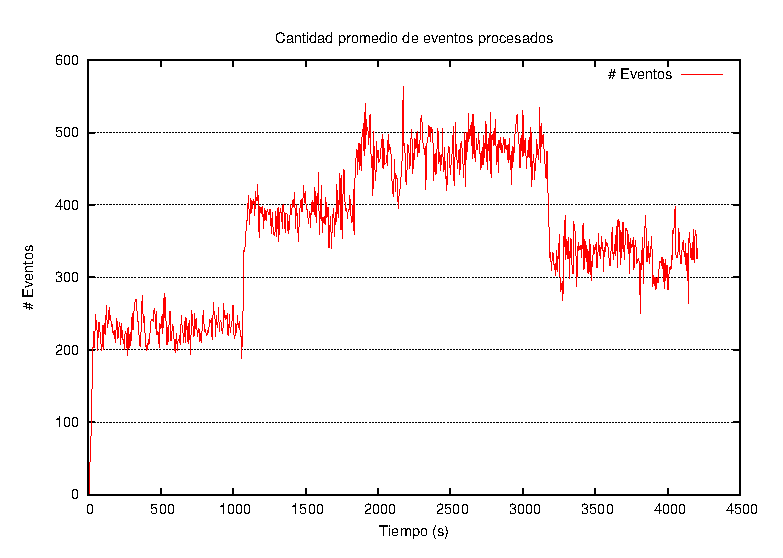
\includegraphics[width=\textwidth]{images/exp/app1/normal/cm/avgEventProcess.eps}
%    \caption{Cantidad promedio de eventos procesados en cada per\'iodo en la primera aplicaci\'on con un env\'io variable de la fuente de datos con uso del modelo.}
%    \label{fig:app1-normal-cm-avgEventProcess}
%\end{minipage}
%\hspace*{1cm}
%\begin{minipage}[c]{0.45\textwidth}
%\centering
%    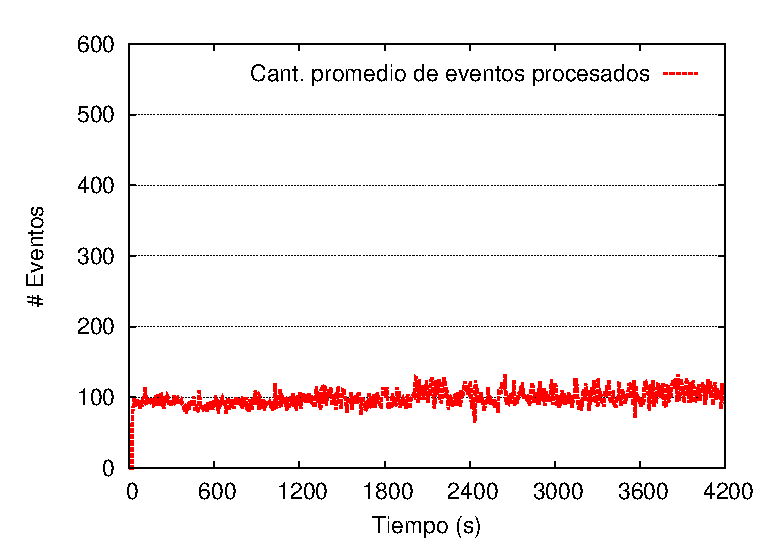
\includegraphics[width=\textwidth]{images/exp/app1/normal/sm/avgEventProcess.eps}
%    \caption{Cantidad promedio de eventos procesados en cada per\'iodo en la primera aplicaci\'on con un env\'io variable de la fuente de datos sin uso del modelo.}
%    \label{fig:app1-normal-sm-avgEventProcess}
%\end{minipage}
%
%\end{figure}

%%% EXP1-VARIABLE PERFORMANCE %%%
Las Figuras \ref{fig:app1-normal-processSystem-cm} y \ref{fig:app1-normal-processSystem-sm} \normalsize{corresponden al segundo experimento y muestra el rendimiento que posee el sistema, y como var\'ia la cantidad de r\'eplicas totales del grafo seg\'un el flujo de datos.} En la Figura \ref{fig:app1-normal-processSystem-cm} \normalsize{se muestra como el sistema fue adaptando la cantidad de r\'eplicas seg\'un la tasa de entrada, de tal manera de modificar la cantidad de r\'eplicas seg\'un la necesidad que se posea. Por ejemplo, en el primer y segundo tercio aumenta la cantidad de r\'eplicas, no as\'i en el \'ultimo, donde disminuye la cantidad de r\'eplicas, debido que existe un exceso en la cantidad de recursos. El promedio en la tasa de salida en esta prueba es de 72 eventos por segundo.} Por otra parte, en la Figura \ref{fig:app1-normal-processSystem-sm} \normalsize{existe una tasa de salida constante, lo cual refleja la nula adaptabilidad del sistema seg\'un el flujo entrante, habiendo un promedio de 19 eventos procesados por segundo. De los resultados presentados, se puede observar una clara mejora en el rendimiento, alcanzado a procesar hasta 3 veces m\'as eventos que la versi\'on sin el modelo el\'astico.}

\begin{figure}[!ht]
	\centering
	\captionsetup{justification=centering}
	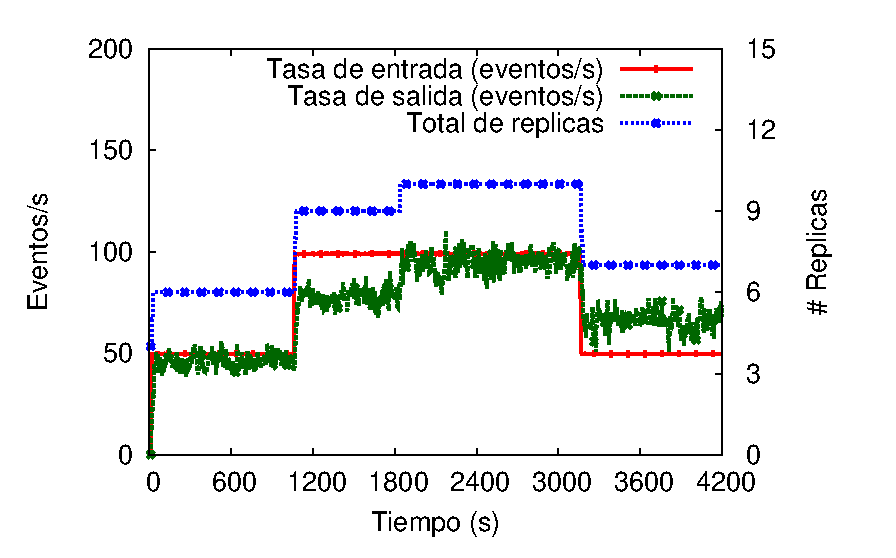
\includegraphics[scale=0.7]{images/exp/app1/normal/cm/processSystem.eps}
    \caption[Rendimiento y cantidad de r\'eplicas totales del grafo en la primera aplicaci\'on con env\'io variable de la fuente de datos con uso del modelo.]{Rendimiento y cantidad de r\'eplicas totales del grafo en la primera aplicaci\'on con env\'io variable de la fuente de datos con uso del modelo.\\Fuente: Elaboraci\'on propia.}
	\label{fig:app1-normal-processSystem-cm}
\end{figure}

\begin{figure}[!ht]
	\centering
	\captionsetup{justification=centering}
	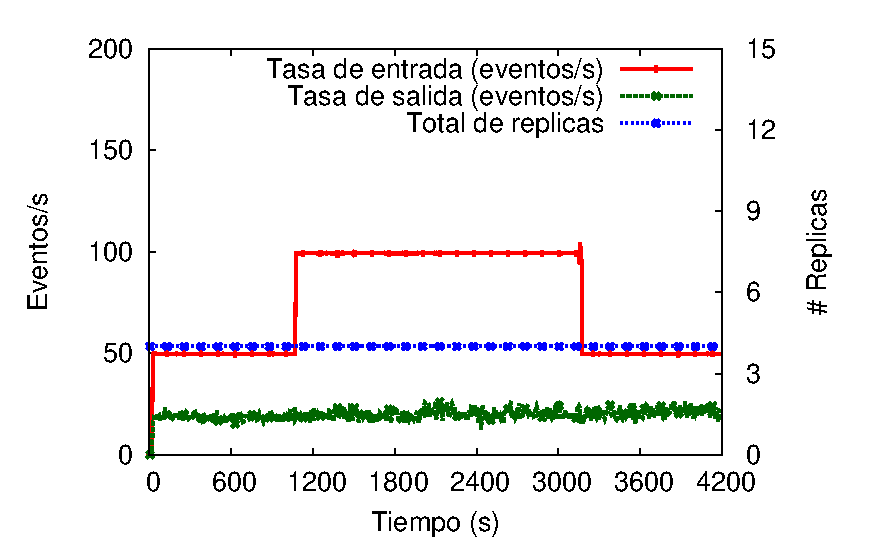
\includegraphics[scale=0.7]{images/exp/app1/normal/sm/processSystem.eps}
    \caption[Rendimiento y cantidad de r\'eplicas totales del grafo en la primera aplicaci\'on con env\'io variable de la fuente de datos sin uso del modelo.]{Rendimiento y cantidad de r\'eplicas totales del grafo en la primera aplicaci\'on con env\'io variable de la fuente de datos sin uso del modelo.\\Fuente: Elaboraci\'on propia.}
	\label{fig:app1-normal-processSystem-sm}
\end{figure}

%%% EXP1-VARIABLE EVENTOS TOTALES %%%
Por otra parte, la cantidad total de eventos procesados en el experimento, se observa en las Figuras \ref{fig:app1-normal-eventCount-cm} y \ref{fig:app1-normal-eventCount-sm} con y sin uso del modelo respectivamente. En el primer gr\'afico se observa variaciones en la curva en el segundo 1100 y 3200, lo cual son los segundos en los cuales hubo un cambio en el flujo de la fuente de datos, por lo que aumenta y disminuye respectivamente la tasa de llegada. En cambio, en el segundo gr\'afico no se aprecia esto, debido que independiente de la tasa de llegada, el procesamiento del sistema es constante, sin adaptarse el sistema a la carga que posea cada operador con el transcurso del tiempo. El sistema con uso del modelo procesa un total de 303.156, contra 82.770 eventos en total sin uso del modelo, lo cual significa un aumento de 3 veces m\'as eventos procesados.

\begin{figure}[!ht]
	\centering
	\captionsetup{justification=centering}
    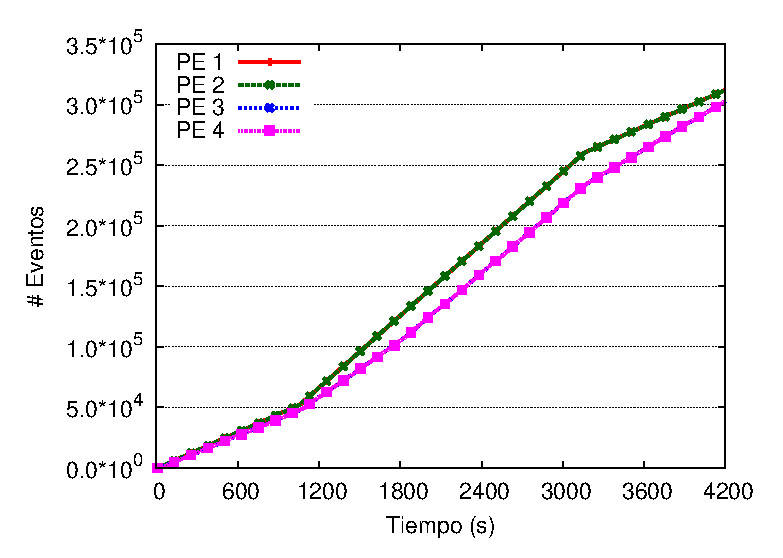
\includegraphics[scale=0.7]{images/exp/app1/normal/cm/eventCount.eps}
    \caption[Cantidad total de eventos procesados en la primera aplicaci\'on con un env\'io variable de la fuente de datos con uso del modelo.]{Cantidad total de eventos procesados en la primera aplicaci\'on con un env\'io variable de la fuente de datos con uso del modelo.\\Fuente: Elaboraci\'on propia.}
    \label{fig:app1-normal-eventCount-cm}
\end{figure}

\begin{figure}[!ht]
	\centering
	\captionsetup{justification=centering}
    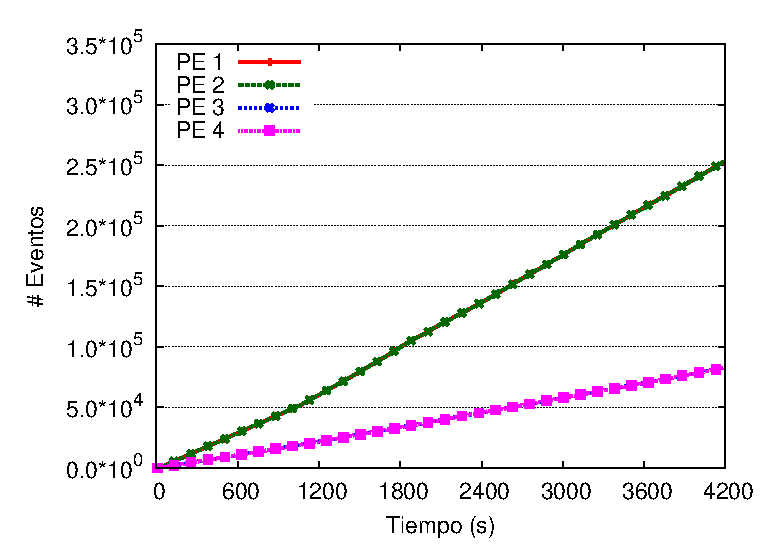
\includegraphics[scale=0.7]{images/exp/app1/normal/sm/eventCount.eps}
    \caption[Cantidad total de eventos procesados en la primera aplicaci\'on con un env\'io variable de la fuente de datos sin uso del modelo.]{Cantidad total de eventos procesados en la primera aplicaci\'on con un env\'io variable de la fuente de datos sin uso del modelo.\\Fuente: Elaboraci\'on propia.}
    \label{fig:app1-normal-eventCount-sm}
\end{figure}

\subsection{Aplicaci\'on 2: Contador de palabras en muestras de textos}
En la segunda aplicaci\'on se ha procedido a realizar dos experimentos, los cuales son similares a los anteriores. En el primer experimento se realiza un env\'io constante de los eventos, y en el segundo, un env\'io variable. En ambos experimentos, se han realizado dos pruebas, donde la primera consiste en la ejecuci\'on de la aplicaci\'on en un sistema SPS que usa el modelo el\'astico, y la segunda sin el uso de \'este.

\normalsize{Para el an\'alisis de los experimentos, se ha considerado el rendimiento y la cantidad de r\'eplicas del grafo y la cantidad total de eventos procesados. En el Anexo} \ref{apendice:estadisticas-operadores} \normalsize{se presentan las estad\'isticas de cada uno de los operadores.}

%%% EXP2 CONSTANTE - OPERADORES %%%

%En las Figuras \ref{fig:app2-uniform-statusSplitPE-cm} y \ref{fig:app2-uniform-statusSplitPE-sm} se observan las estad\'isticas del PE Split con y sin uso del modelo respectivamente con un flujo constante de eventos. En el primer gr\'afico la tasa de llegada de los primeros 200 segundos se encuentran ciertos \textit{peak}, los cuales se deben al retraso en la toma de estad\'isticas, producto de la replicaci\'on del PE Counter como se aprecia en la Figura \ref{fig:app2-uniform-statusCounterPE-cm}. Independiente del uso del modelo, se observa que el comportamiento entre los dos PEs es pr\'acticamente igual, y eso se debe a la baja carga que posee el PE. Esto se debe a que este operador es auxiliar, por lo que el costo de separar las palabras y enviarlo a las distintas r\'eplicas del siguiente operador, el cual posee estado, es de bajo costo computacional.
%
%En cambio, en las Figuras \ref{fig:app2-uniform-statusCounterPE-cm} y \ref{fig:app2-uniform-statusCounterPE-sm} se observa una diferencia en los rendimientos del PE Counter. Esto se debe a que este operador posee un alto costo computacional, debido al gran tama\~no de la bolsa de palabras que se usa para comparar con las palabras del \textit{tweets}. Debido a esto, al generar las r\'eplicas, se produce una mejora considerable del operador en los primeros 100 segundo.
%
%En este caso, el predictor se activa dado que se realiza un aumento de 9 a 14 r\'eplicas. Si bien, la cantidad de r\'eplicas fue alta, no se considera el operador en estado ocioso, dado que el promedio de tasa de procesamiento posterior al segundo 100 es de 0.63, por lo que no se disminuye la cantidad de r\'eplicas.
%
%Dentro de las observaciones importantes a destacar, se encuentra el procesamiento del PE Counter, el cual al procesar los eventos, deja algunos en cola para posteriormente ser procesados, independiente si se a\~naden m\'as r\'eplicas, lo cual se puede observar en la cola que se muestra en la Figura \ref{fig:app2-uniform-statusCounterPE-cm}. Si bien, se generan colas con el uso del modelo, es menos de la mitad de las colas que surgen sin el uso del modelo. Este problema surge debido a la implementaci\'on en el SPS S4, debido que los PEs no procesan la cantidad de eventos que deben procesar en un per\'iodo de tiempo. Esto no significa que se pierden eventos, sino que en caso de no procesarlos los deja en cola para posteriormente procesarlos. Por lo que si no se env\'ian m\'as eventos de la fuente de datos, los eventos en cola se procesan hasta vaciar el \textit{buffer}.
%
%En el \'ultimo PE, se observa que existe una baja cantidad de eventos entrantes, como se muestra en las Figuras \ref{fig:app2-uniform-statusMergePE-cm} y \ref{fig:app2-uniform-statusMergePE-sm}, debido a su condici\'on de operador auxiliar. Cabe recordar que se denomina operador auxiliar a los PEs predecesor y sucesores del posible operador sobrecargado, de esta manera, estos operadores se dedican a dividir la informaci\'on para enviarla a las distintas r\'eplicas del operador, y posteriormente juntar la informaci\'on obtenida por las distintas r\'eplicas de \'este. La baja cantidad de eventos entrantes se debe a que los eventos entrantes s\'olo son enviados cada 10 segundos por el PE Counter. En el primer gr\'afico, se observa que la tasa de llegada aumenta posterior a los 100 segundos, debido a la replicaci\'on del operador predecesor. En cambio, en el segundo gr\'afico, el flujo de entrada s\'olo se condiciona por una r\'eplica, por lo que no existe un aumento de la tasa de llegada. Cabe destacar que el sistema con modelo si genera colas, a diferencia del sin modelo, y esto se debe a que al procesar mayor cantidad de eventos, surge el problema de procesamiento descrito anteriormente, debido a la implementaci\'on realizada en el SPS S4.

%\begin{figure}[p]
%\centering
%    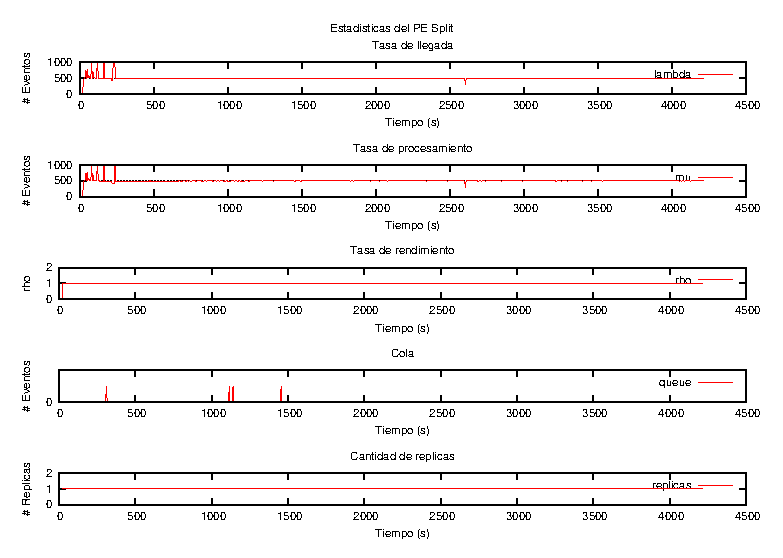
\includegraphics[scale=1.1]{images/exp/app2/uniform/cm/statusSplitPE.eps}
%    \caption{Estad\'isticas del PE Split en la segunda aplicaci\'on con un env\'io constante de la fuente de datos con uso del modelo.}
%    \label{fig:app2-uniform-statusSplitPE-cm}
%\end{figure}
%
%\begin{figure}[p]
%\centering
%    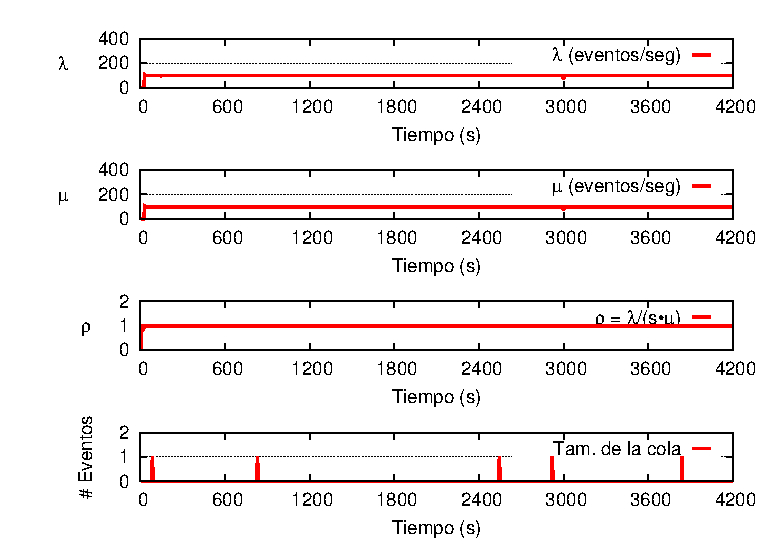
\includegraphics[scale=1.1]{images/exp/app2/uniform/sm/statusSplitPE.eps}
%    \caption{Estad\'isticas del PE Split en la segunda aplicaci\'on con un env\'io constante de la fuente de datos sin uso del modelo.}
%    \label{fig:app2-uniform-statusSplitPE-sm}
%\end{figure}
%
%\begin{figure}[p]
%\centering
%    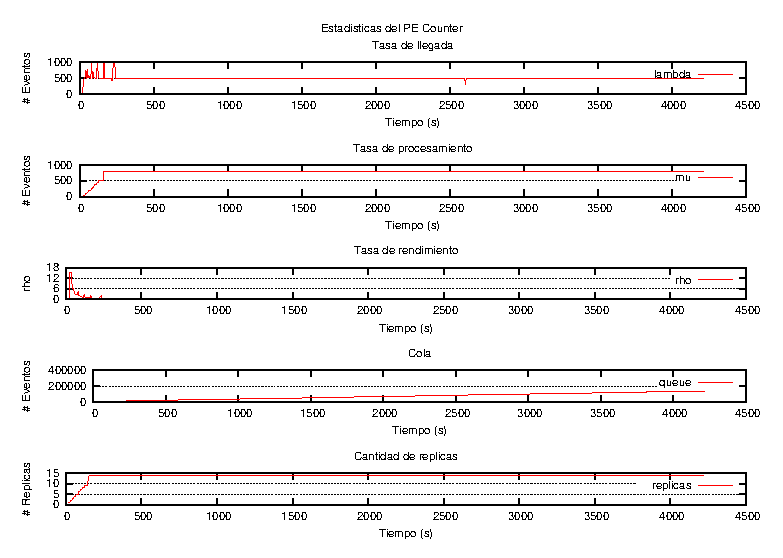
\includegraphics[scale=1.1]{images/exp/app2/uniform/cm/statusCounterPE.eps}
%    \caption{Estad\'isticas del PE Counter en la segunda aplicaci\'on con un env\'io constante de la fuente de datos con uso del modelo.}
%    \label{fig:app2-uniform-statusCounterPE-cm}
%\end{figure}
%
%\begin{figure}[p]
%\centering
%    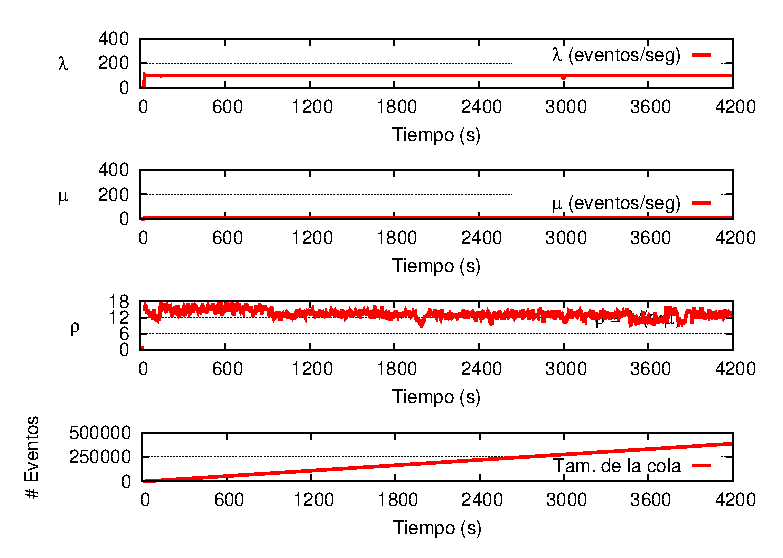
\includegraphics[scale=1.1]{images/exp/app2/uniform/sm/statusCounterPE.eps}
%    \caption{Estad\'isticas del PE Counter en la segunda aplicaci\'on con un env\'io constante de la fuente de datos sin uso del modelo.}
%    \label{fig:app2-uniform-statusCounterPE-sm}
%\end{figure}
%
%\begin{figure}[p]
%\centering
%    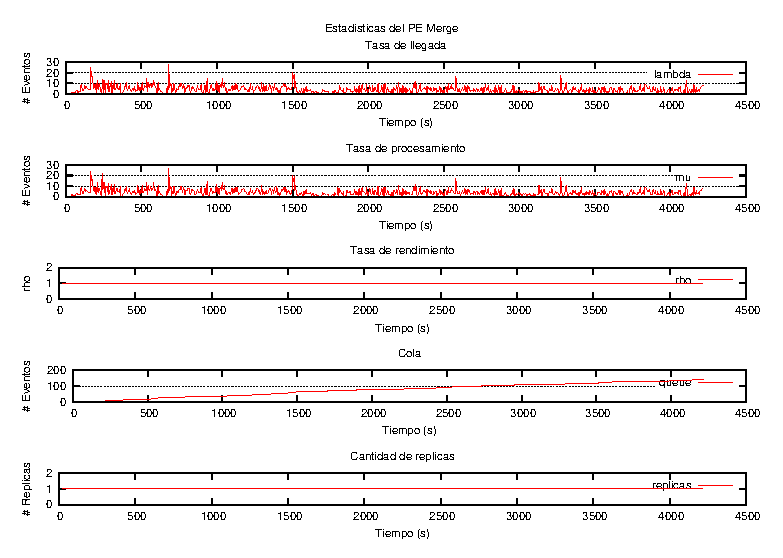
\includegraphics[scale=1.1]{images/exp/app2/uniform/cm/statusMergePE.eps}
%    \caption{Estad\'isticas del PE Merge en la segunda aplicaci\'on con un env\'io constante de la fuente de datos con uso del modelo.}
%    \label{fig:app2-uniform-statusMergePE-cm}
%\end{figure}
%
%\begin{figure}[p]
%\centering
%    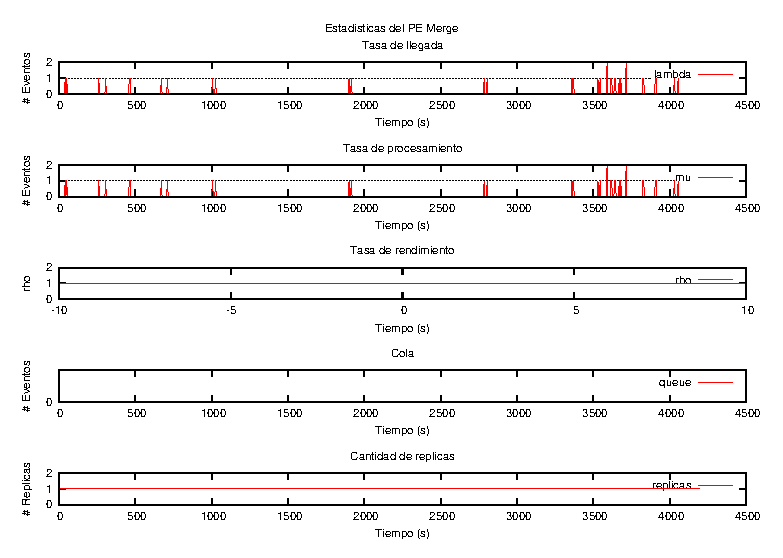
\includegraphics[scale=1.1]{images/exp/app2/uniform/sm/statusMergePE.eps}
%    \caption{Estad\'isticas del PE Merge en la segunda aplicaci\'on con un env\'io constante de la fuente de datos sin uso del modelo.}
%    \label{fig:app2-uniform-statusMergePE-sm}
%\end{figure}

%%% EXP2 CONSTANTE - PERFORMANCE %%%

La Figura \ref{fig:app2-uniform-processSystem-cm} \normalsize{corresponde al primer experimento y muestra el flujo de datos entrantes del sistema, y como var\'ia la cantidad de r\'eplicas totales del grafo seg\'un el flujo de datos.} En esta figura \normalsize{se observa que al principio de la ejecuci\'on de la aplicaci\'on, existen altas variaciones con el flujo de eventos entrante, y eso se debe a que al crear una r\'eplica del operador sobrecargado, el PE Counter} (v\'ease Anexo \ref{apendice:estadisticas-operadores}), \normalsize{genera una sobrecarga a nivel f\'isico en la m\'aquina, habiendo retrasos en el procesamiento de los datos, lo cual no afecta en el an\'alisis del grafo l\'ogico. Por otra parte, en este experimento se muestra una replicaci\'on basado en el algoritmo predictivo, lo cual se debe al an\'alisis del rendimiento del operador seg\'un la tasa de rendimiento del PE Counter.}

\begin{figure}[!ht]
	\centering
	\captionsetup{justification=centering}
	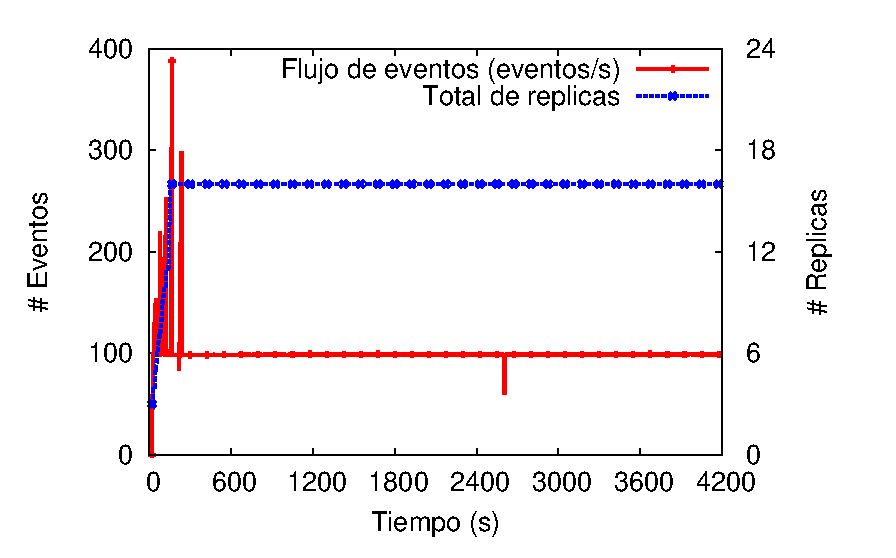
\includegraphics[scale=0.7]{images/exp/app2/uniform/cm/processSystem.eps}
    \caption[Flujo de datos y cantidad de r\'eplicas totales del grafo en la primera aplicaci\'on con env\'io variable de la fuente de datos con uso del modelo.]{Flujo de datos y cantidad de r\'eplicas totales del grafo en la primera aplicaci\'on con env\'io variable de la fuente de datos con uso del modelo.\\Fuente: Elaboraci\'on propia.}
	\label{fig:app2-uniform-processSystem-cm}
\end{figure}

%\begin{figure}[!ht]
%	\centering
%	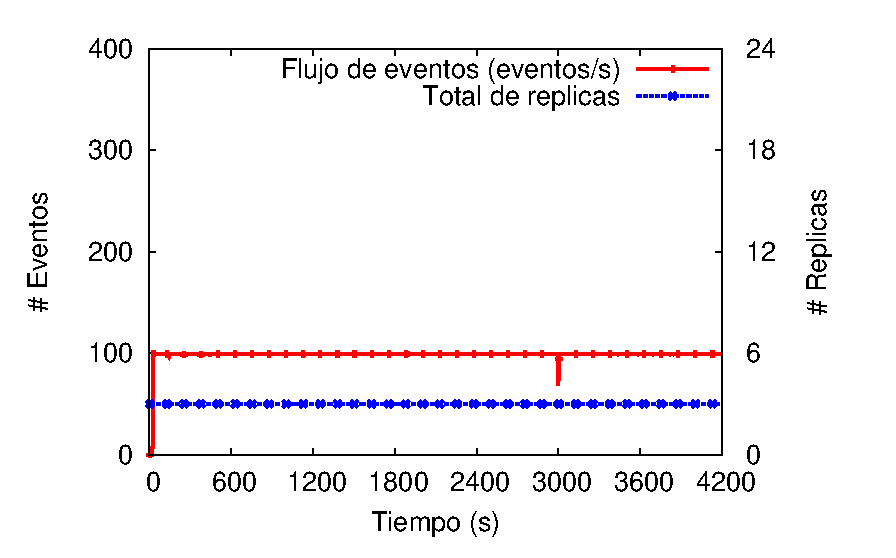
\includegraphics[scale=0.7]{images/exp/app2/uniform/sm/processSystem.eps}
%    \caption{Rendimiento y cantidad de r\'eplicas totales del grafo en la primera aplicaci\'on con env\'io variable de la fuente de datos sin uso del modelo.}
%	\label{fig:app2-uniform-processSystem-sm}
%\end{figure}

%%% EXP2 CONSTANTE - EVENTOS TOTALES %%%

Por otra parte, en las Figuras \ref{fig:app2-uniform-eventCount-cm} y \ref{fig:app2-uniform-eventCount-sm} se muestra la cantidad total de eventos procesados. En el primer gr\'afico se observa que la diferencia de la pendiente entre las rectas del primer y segundo PE, es menor que en el segundo gr\'afico. Esto se debe al aumento de la cantidad de r\'eplicas, por lo que se puede procesar mayor cantidad de eventos, alcanzando un total de 275.290 eventos con uso el modelo contra 28.152 sin uso del modelo. En este caso se logro procesar hasta 9 veces mas eventos haciendo uso del modelo el\'astico.

Dentro de las observaciones importantes est\'a lo ocurrido en la Figura \ref{fig:app2-uniform-eventCount-cm}, donde no existe una mejora por parte del segundo PE de manera paralela al flujo de datos emanado por el primer PE. Como se hab\'ia explicado anteriormente, independiente que se generen m\'as r\'eplicas, los operadores igualmente van a encolar debido a la sobrecarga surgida por parte de la m\'aquina f\'isica.

En el PE 3 (PE Merge) se presenta una baja cantidad de eventos procesados, lo cual se observa en las Figuras \ref{fig:app2-uniform-eventCount-cm} y \ref{fig:app2-uniform-eventCount-sm}. Esto se debe a su condici\'on de operador auxiliar. Cabe recordar que se denomina operador auxiliar a los PEs predecesor y sucesores de un operador con estado, de esta manera, estos operadores se dedican a dividir la informaci\'on para enviarla a las distintas r\'eplicas del operador, y posteriormente juntar la informaci\'on obtenida por las distintas r\'eplicas de \'este. La baja cantidad de eventos entrantes se debe a que los eventos entrantes s\'olo son enviados cada 10 segundos por el PE 2 (PE Counter), y en caso de procesar mayor cantidad de datos y poseer mayor cantidad de r\'eplicas de este operador, mayor es la cantidad de eventos procesados por el PE 3. Por \'ultimo, en la aplicaci\'on con uso del modelo el\'astico se han procesado 3.491 eventos, contra 34 eventos procesados sin el modelo el\'astico.

\begin{figure}[!ht]
	\centering
	\captionsetup{justification=centering}
    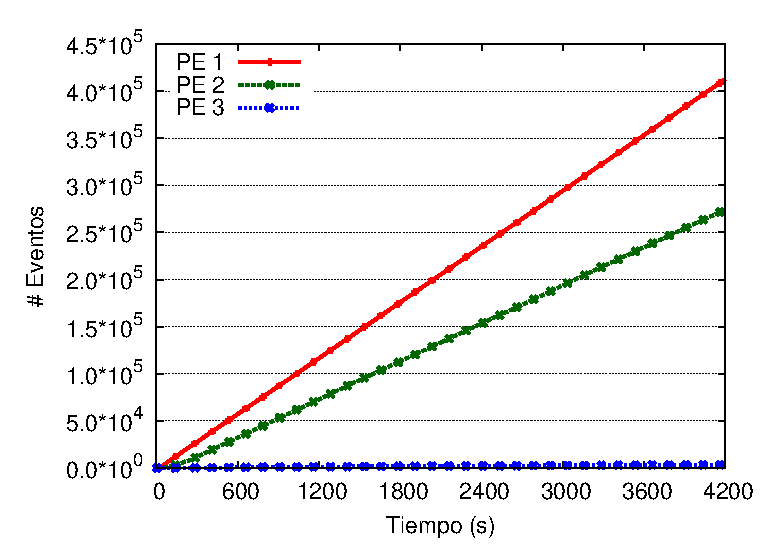
\includegraphics[scale=0.7]{images/exp/app2/uniform/cm/eventCount.eps}
    \caption[Cantidad total de eventos procesados en la segunda aplicaci\'on con un env\'io constante de la fuente de datos sin uso del modelo.]{Cantidad total de eventos procesados en la segunda aplicaci\'on con un env\'io constante de la fuente de datos sin uso del modelo.\\Fuente: Elaboraci\'on propia.}
    \label{fig:app2-uniform-eventCount-cm}
\end{figure}

\begin{figure}[!ht]
	\centering
	\captionsetup{justification=centering}
    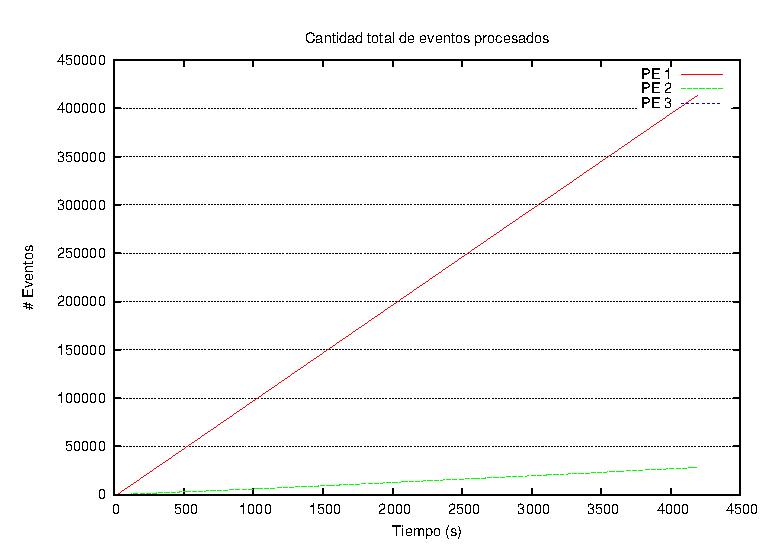
\includegraphics[scale=0.7]{images/exp/app2/uniform/sm/eventCount.eps}
    \caption[Cantidad total de eventos procesados en la segunda aplicaci\'on con un env\'io constante de la fuente de datos con uso del modelo.]{Cantidad total de eventos procesados en la segunda aplicaci\'on con un env\'io constante de la fuente de datos con uso del modelo.\\Fuente: Elaboraci\'on propia.}
    \label{fig:app2-uniform-eventCount-sm}
\end{figure}

%%% EXP2-VARIACIONES OPERADORES %%%

%En las Figuras \ref{fig:app2-uniform-statusSplitPE-cm} y \ref{fig:app2-uniform-statusSplitPE-sm} se observan las estad\'isticas del PE Split con y sin uso del modelo respectivamente con un flujo variable de eventos. Como se mencion\'o anteriormente, en las estad\'isticas recuperadas de la aplicaci\'on haciendo uso del modelo se pueden observar \textit{peaks}, los cuales son provocados por la replicaci\'on del siguiente operador. Sin embargo, estos \textit{peaks} no impactan el rendimiento del sistema haciendo uso del modelo propuesto. Debido que el PE Split posee un bajo nivel de c\'omputo, no existe una tasa de rendimiento que sea inestable, tanto para el sistema con y sin uso del modelo, por lo que no se presentan sobrecargas.
%
%A diferencia del PE Split, en el PE Counter si existe un nivel de sobrecarga, como se observar en las Figuras \ref{fig:app2-normal-statusCounterPE-cm} y \ref{fig:app2-normal-statusCounterPE-sm}. En el primer gr\'afico se aprecia que en los primeros 100 segundos existe una inestabilidad en el sistema, sin embargo, posteriormente se alcanza estabilidad utilizando el modelo, dado que se replica el operador. Esta inestabilidad se vuelve a apreciar en el segundo 1100, cuando aumenta el env\'io de eventos desde la fuente de datos, lo cual hace que la cantidad de r\'eplicas existentes sean insuficientes, volviendo a replicar el operador. Y finalmente, en el \'ultimo tramo disminuye la cantidad de r\'eplicas en el segundo 3200, debido que el env\'io de datos disminuye.
%
%Como se explic\'o en el experimento de env\'io variable de la fuente de datos en la aplicaci\'on 1, la cantidad \'optima de operadores en el primer tramo es distinta a la del tercer tramo. Esto se debe a que en el primer tramo aumenta la cantidad de r\'eplicas para ir convergiendo $\rho$ a un valor de 1, en cambio, en el tercer tramo disminuye la cantidad de r\'eplicas para ir convergiendo $\rho$ a 0.5, l\'imite inferior para definir el estado estable.
%
%Por otra parte, en este experimento no se ha activado el predictor, y esto se debe a que la replicaci\'on fue paulatina. Por lo tanto, el operador alcanza una convergencia de la cantidad de r\'eplicas necesarias, por lo que al predecir se determina que el operador se encuentra estable a futuro.
%
%En el tercer PE, se analiza que la tasa de llegada es baja tanto en las Figuras \ref{fig:app2-normal-statusMergePE-cm} y \ref{fig:app2-normal-statusMergePE-sm}, y esto se debe a que este PE es auxiliar como se explic\'o en el anterior experimento, por lo que le llegan eventos cada 10 segundos por cada r\'eplica del PE Counter. El an\'alisis que se realiza en el PE Merge es el mismo explicado en el anterior experimento, donde la tasa de llegada va a depender de la cantidad de r\'eplicas existentes en el PE Counter, por lo que la tasa de llegada es mayor en el sistema con modelo.

%\begin{figure}[p]
%\centering
%    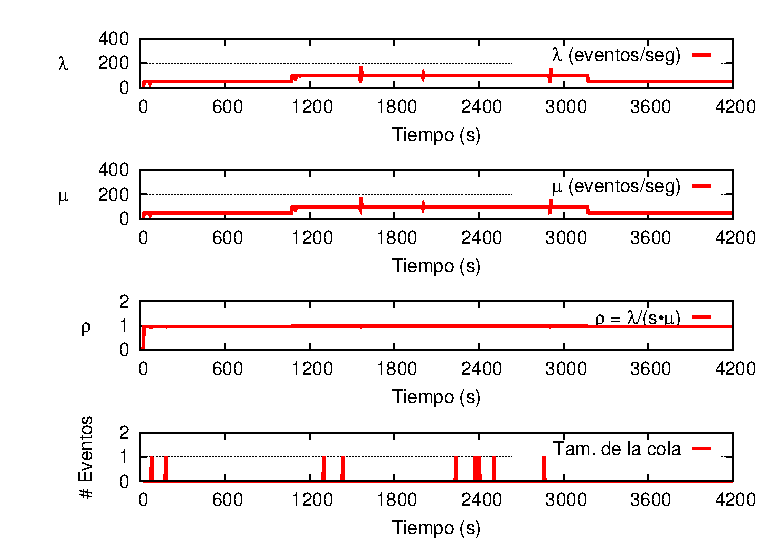
\includegraphics[scale=1.1]{images/exp/app2/normal/cm/statusSplitPE.eps}
%    \caption{Estad\'isticas del PE Split en la segunda aplicaci\'on con un env\'io variable de la fuente de datos con uso del modelo.}
%    \label{fig:app2-normal-statusSplitPE-cm}
%\end{figure}
%
%\begin{figure}[p]
%\centering
%    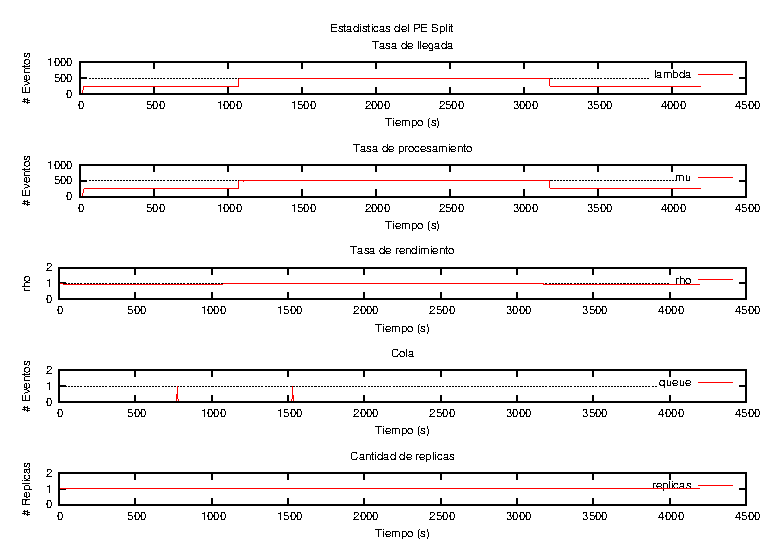
\includegraphics[scale=1.1]{images/exp/app2/normal/sm/statusSplitPE.eps}
%    \caption{Estad\'isticas del PE Split en la segunda aplicaci\'on con un env\'io variable de la fuente de datos sin uso del modelo.}
%    \label{fig:app2-normal-statusSplitPE-sm}
%\end{figure}
%
%\begin{figure}[p]
%\centering
%    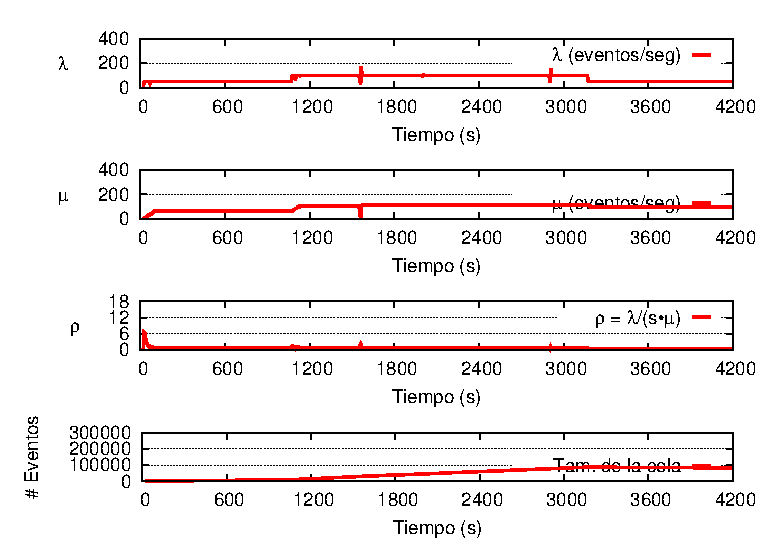
\includegraphics[scale=1.1]{images/exp/app2/normal/cm/statusCounterPE.eps}
%    \caption{Estad\'isticas del PE Counter en la segunda aplicaci\'on con un env\'io variable de la fuente de datos con uso del modelo.}
%    \label{fig:app2-normal-statusCounterPE-cm}
%\end{figure}
%
%\begin{figure}[p]
%\centering
%    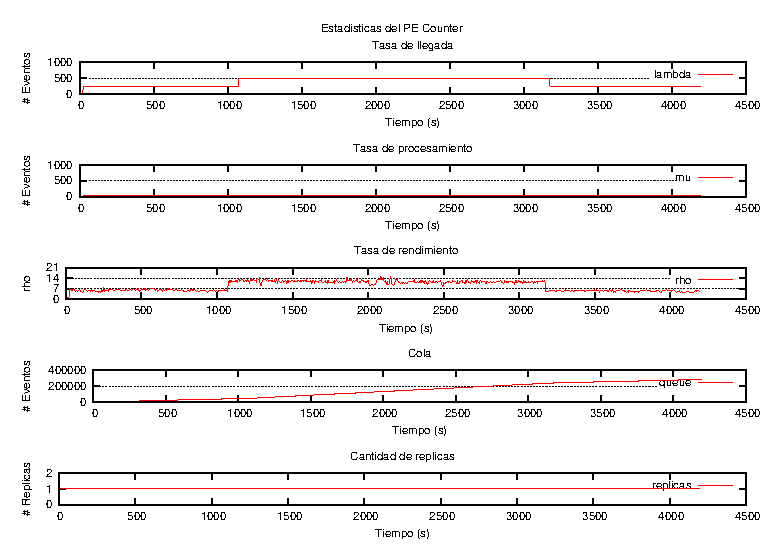
\includegraphics[scale=1.1]{images/exp/app2/normal/sm/statusCounterPE.eps}
%    \caption{Estad\'isticas del PE Counter en la segunda aplicaci\'on con un env\'io variable de la fuente de datos sin uso del modelo.}
%    \label{fig:app2-normal-statusCounterPE-sm}
%\end{figure}
%
%\begin{figure}[p]
%\centering
%    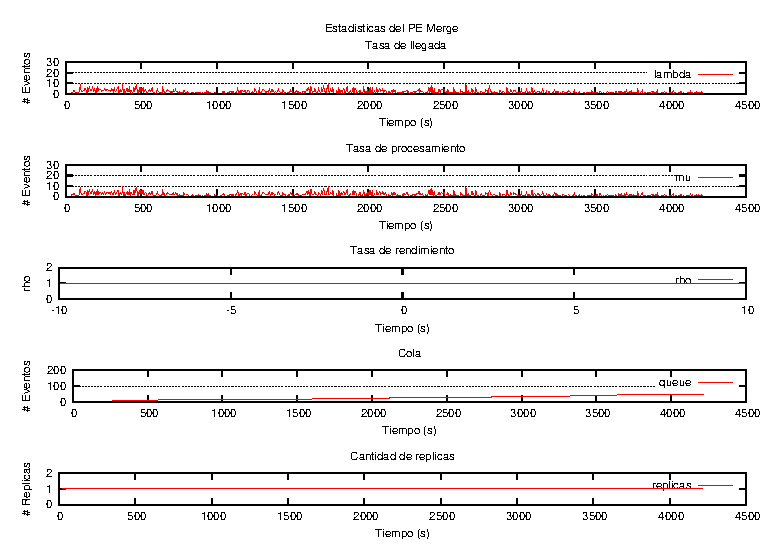
\includegraphics[scale=1.1]{images/exp/app2/normal/cm/statusMergePE.eps}
%    \caption{Estad\'isticas del PE Merge en la segunda aplicaci\'on con un env\'io variable de la fuente de datos con uso del modelo.}
%    \label{fig:app2-normal-statusMergePE-cm}
%\end{figure}
%
%\begin{figure}[p]
%\centering
%    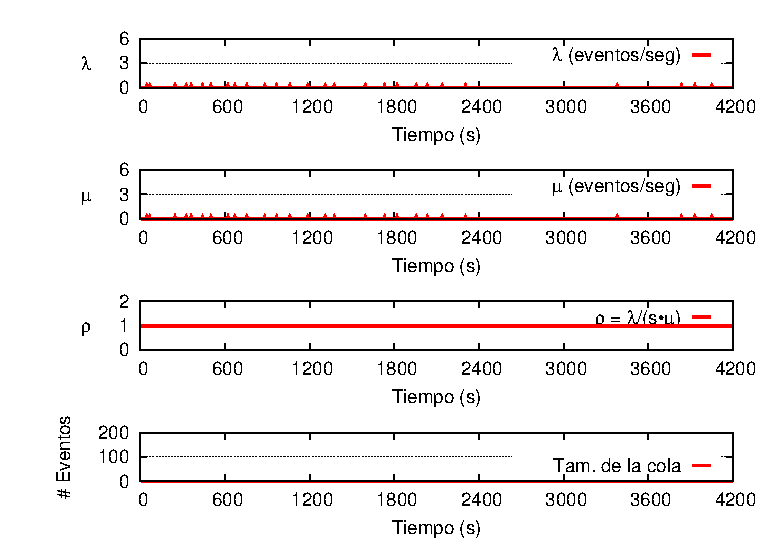
\includegraphics[scale=1.1]{images/exp/app2/normal/sm/statusMergePE.eps}
%    \caption{Estad\'isticas del PE Merge en la segunda aplicaci\'on con un env\'io variable de la fuente de datos sin uso del modelo.}
%    \label{fig:app2-normal-statusMergePE-sm}
%\end{figure}

%%% EXP2-VARIABLE PERFORMANCE %%%

La Figura \ref{fig:app2-normal-processSystem-cm} \normalsize{corresponde al primer experimento y muestra el flujo de datos entrantes del sistema, y como var\'ia la cantidad de r\'eplicas totales del grafo seg\'un el flujo de datos.} En esta figura \normalsize{se puede observar como el n\'umero de r\'eplicas se adapta al tr\'afico recibido. En el primer y segundo tercio se muestra un aumento de r\'eplicas, pero posteriormente en el \'ultimo disminuye, aprovechando los recursos que se disponen. A diferencia del experimento anterior, en \'este no se activa el algoritmo predictivo, y eso se debe a qu\'e no existe una posible sobrecarga a futuro, dado que se estabiliza el sistema antes de este an\'alisis debido al algoritmo reactivo.}

\begin{figure}[!ht]
	\centering
	\captionsetup{justification=centering}
	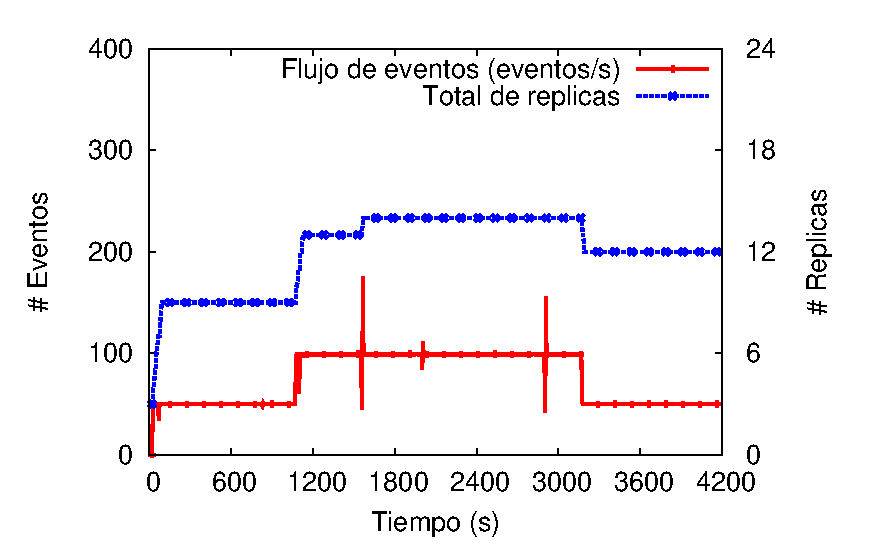
\includegraphics[scale=0.7]{images/exp/app2/normal/cm/processSystem.eps}
    \caption[Flujo de datos y cantidad de r\'eplicas totales del grafo en la primera aplicaci\'on con env\'io variable de la fuente de datos con uso del modelo.]{Flujo de datos y cantidad de r\'eplicas totales del grafo en la primera aplicaci\'on con env\'io variable de la fuente de datos con uso del modelo.\\Fuente: Elaboraci\'on propia.}
	\label{fig:app2-normal-processSystem-cm}
\end{figure}

%%% EXP2-VARIABLE EVENTOS TOTALES %%%

Por otro lado, en las Figuras \ref{fig:app2-normal-eventCount-cm} y \ref{fig:app2-normal-eventCount-sm} se muestra la cantidad total de eventos procesados. En el primer gr\'afico se aprecia que la curva del primer PE y el segundo PE es m\'as cercana que las del segundo gr\'afico, y esto se debe a la replicaci\'on que se ha efectuado en el sistema. Cabe destacar que el sistema con uso del modelo ha procesado un total de 228.942 eventos, mientras que el sistema sin uso del modelo ha procesado 27.751 eventos. Por lo que la soluci\'on permite aumentar en m\'as de 8 veces la cantidad de eventos procesados.

El an\'alisis que se realiza en el PE 3 (PE Merge) es el mismo explicado en el anterior experimento, donde la cantidad de eventos procesados va a depender de la cantidad de r\'eplicas existentes en el PE 2 (PE Counter). Por \'ultimo, se ha realizado un procesamiento de 1.578 eventos con uso del modelo, y 27 eventos sin uso del modelo.

\begin{figure}[!ht]
	\centering
	\captionsetup{justification=centering}
    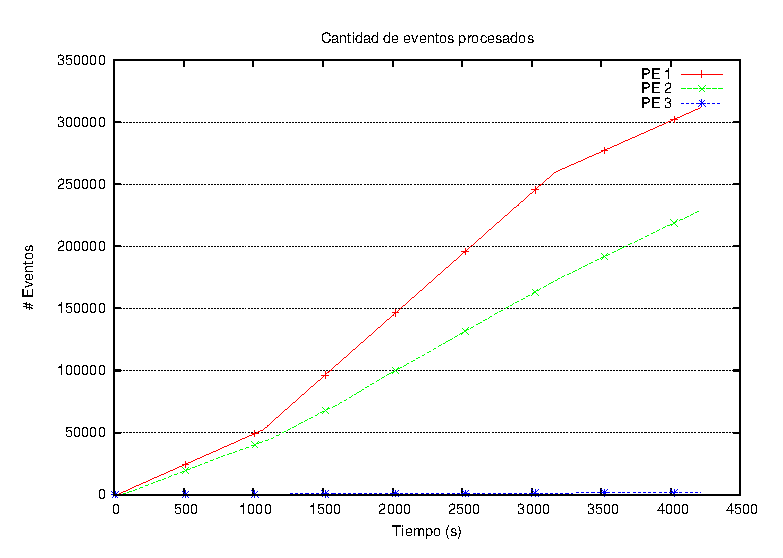
\includegraphics[scale=0.7]{images/exp/app2/normal/cm/eventCount.eps}
    \caption[Cantidad total de eventos procesados en la segunda aplicaci\'on con un env\'io variable de la fuente de datos con uso del modelo.]{Cantidad total de eventos procesados en la segunda aplicaci\'on con un env\'io variable de la fuente de datos con uso del modelo.\\Fuente: Elaboraci\'on propia.}
    \label{fig:app2-normal-eventCount-cm}
\end{figure}

\begin{figure}[!ht]
	\centering
	\captionsetup{justification=centering}
    \includegraphics[scale=0.7]{images/exp/app2/normal/sm/eventCount.eps}
    \caption[Cantidad total de eventos procesados en la segunda aplicaci\'on con un env\'io variable de la fuente de datos sin uso del modelo.]{Cantidad total de eventos procesados en la segunda aplicaci\'on con un env\'io variable de la fuente de datos sin uso del modelo.\\Fuente: Elaboraci\'on propia.}
    \label{fig:app2-normal-eventCount-sm}
\end{figure}

\subsection{Aplicaci\'on 3: Aplicaci\'on sint\'etica}
En la tercera aplicaci\'on se ha procedido a realizar un experimento que consta de dos pruebas, al igual que en las anteriores pruebas, donde una de ellas hace uso del modelo el\'astico y la otra no. Ambas pruebas se han realizado con un env\'io constante de 100 eventos por segundo desde la fuente de datos.

Para el an\'alisis de los experimentos, se ha considerado el consumo de memoria, el uso de la CPU, \normalsize{el rendimiento, la cantidad de r\'eplicas del grafo} y la cantidad total de eventos procesados. En el Anexo \ref{apendice:estadisticas-operadores} \normalsize{se presentan las estad\'isticas de cada uno de los operadores.}

%%% EXP3 - CPU %%%

Respecto a la utilizaci\'on de CPU, se puede observar en las Figuras \ref{fig:app3-consumeCPU-cm} y \ref{fig:app3-consumeCPU-sm} el porcentaje de uso con y sin uso del modelo respectivamente. Si bien la diferencia no es significante en el uso de la CPU por parte de la aplicaci\'on, en el primer caso existe un promedio de $0.62\%$ de utilizaci\'on de CPU, contra un promedio de $0.61\%$ de uso en el segundo caso, habiendo un aumento del $0,01\%$ de utilizaci\'on promedio de CPU. Dentro de los primeros 10 segundo existe un alto uso de CPU en ambos gr\'aficos, lo que se debe al despliegue y compilaci\'on de la aplicaci\'on en el sistema de S4.

\begin{figure}[!ht]
	\centering
	\captionsetup{justification=centering}
    \includegraphics[scale=0.65]{images/exp/app3/cm/fisical/consumeCPU.eps}
    \caption[Porcentaje de utilizaci\'on de la CPU en la tercera aplicaci\'on con uso del modelo.]{Porcentaje de utilizaci\'on de la CPU en la tercera aplicaci\'on con uso del modelo.\\Fuente: Elaboraci\'on propia.}
    \label{fig:app3-consumeCPU-cm}
\end{figure}

\begin{figure}[!ht]
	\centering
	\captionsetup{justification=centering}
    \includegraphics[scale=0.65]{images/exp/app3/sm/fisical/consumeCPU.eps}
    \caption[Porcentaje de utilizaci\'on de la CPU en la tercera aplicaci\'on sin uso del modelo.]{Porcentaje de utilizaci\'on de la CPU en la tercera aplicaci\'on sin uso del modelo.\\Fuente: Elaboraci\'on propia.}
    \label{fig:app3-consumeCPU-sm}
\end{figure}

%%% EXP3 - RAM %%%

Por otra parte, el consumo de memoria RAM es presentado por las Figuras \ref{fig:app3-consumeRAM-cm} y \ref{fig:app3-consumeRAM-sm}, donde la primera es con uso de modelo y la segunda sin uso. En el primer gr\'afico existe un consumo promedio de $264$ MB versus $268$ MB del segundo gr\'afico, habiendo una disminuci\'on del $1,5\%$ de consumo de memoria RAM. En el primer gr\'afico se observa un aumento del consumo de memoria en el segundo 200, a diferencia del segundo gr\'afico, debido al mayor consumo de eventos y creaci\'on de nuevos operadores. Posterior al segundo 600, por parte del sistema sin uso del modelo, se muestra un aumento del consumo de memoria, lo cual se debe a la cantidad de eventos en la cola que existen en el sistema, a diferencia del primer gr\'afico que hubo una convergencia en el consumo de la memoria, por lo que posteriormente al reducir las colas, reduce igualmente el consumo de memoria principal en la ejecuci\'on.

\begin{figure}[!ht]
	\centering
	\captionsetup{justification=centering}
    \includegraphics[scale=0.7]{images/exp/app3/cm/fisical/consumeRAM.eps}
    \caption[Consumo de memoria RAM en la tercera aplicaci\'on con uso del modelo.]{Consumo de memoria RAM en la tercera aplicaci\'on con uso del modelo.\\Fuente: Elaboraci\'on propia.}
    \label{fig:app3-consumeRAM-cm}
\end{figure}

\begin{figure}[!ht]
	\centering
	\captionsetup{justification=centering}
    \includegraphics[scale=0.7]{images/exp/app3/sm/fisical/consumeRAM.eps}
    \caption[Consumo de memoria RAM en la tercera aplicaci\'on sin uso del modelo.]{Consumo de memoria RAM en la tercera aplicaci\'on sin uso del modelo.\\Fuente: Elaboraci\'on propia.}
    \label{fig:app3-consumeRAM-sm}
\end{figure}

%%% EXP3 - PERFORMANCE

En las Figuras \ref{fig:app3-processSystem-cm} y \ref{fig:app3-processSystem-sm} \normalsize{corresponden al rendimiento que posee el sistema, y como \'este var\'ia la cantidad de r\'eplicas totales del grafo seg\'un la tasa de entrada.} En la Figura \ref{fig:app3-processSystem-cm} \normalsize{se observa que existe un incremento en la cantidad de r\'eplicas, debido a la sobrecarga de los operadores del grafo} (v\'ease Anexo \ref{apendice:estadisticas-operadores}), \normalsize{aumentando el rendimiento de \'este, de tal manera de procesar 97 eventos por segundo en promedio con el uso del modelo. En cambio, en la Figura} \ref{fig:app3-processSystem-sm} \normalsize{no existe un aumento en el rendimiento, teniendo una tasa de salida promedio de 33 eventos por segundo. De esta manera, existe una mejora de 2 veces m\'as eventos procesados con el uso del modelo propuesto.}

\begin{figure}[!ht]
	\centering
	\captionsetup{justification=centering}
	\includegraphics[scale=0.7]{images/exp/app3/cm/logical/processSystem.eps}
    \caption[Rendimiento y cantidad de r\'eplicas totales del grafo en la tercera aplicaci\'on con uso del modelo.]{Rendimiento y cantidad de r\'eplicas totales del grafo en la tercera aplicaci\'on con uso del modelo.\\Fuente: Elaboraci\'on propia.}
	\label{fig:app3-processSystem-cm}
\end{figure}

\begin{figure}[!ht]
	\centering
	\captionsetup{justification=centering}
	\includegraphics[scale=0.7]{images/exp/app3/sm/logical/processSystem.eps}
    \caption[Rendimiento y cantidad de r\'eplicas totales del grafo en la tercera aplicaci\'on sin uso del modelo.]{Rendimiento y cantidad de r\'eplicas totales del grafo en la tercera aplicaci\'on sin uso del modelo.\\Fuente: Elaboraci\'on propia.}
	\label{fig:app3-processSystem-sm}
\end{figure}

En cuanto a la cantidad total de eventos procesados, en las Figuras \ref{fig:app3-eventCount-cm} y \ref{fig:app3-eventCount-sm} se aprecia que la cantidad de eventos procesados es mayor en el primero gr\'afico, el cual hace uso del modelo el\'astico. En el primer gr\'afico existe un total de 88.169 eventos procesados y en el segundo un total de 29.714 eventos procesados, existiendo una mejora de 3 veces la cantidad de eventos procesados.

%%% EXP 3 - TIEMPO ALGORITMOS %%%

Finalmente, en la Tabla \ref{tab:tiempo-algoritmos} se muestra el tiempo promedio de ejecuci\'on de cada uno de los algoritmos para el an\'alisis de un operador. Se puede observar que si bien el algoritmo predictivo posee un tiempo de ejecuci\'on mayor que el algoritmo reactivo, no produce un alto costo computacional su implementaci\'on.
>>>>>>> 2593dcc9f1f0f407aaed2b40f87140ab2e858079

\newpage
\begin{table}[!ht]
\centering
\captionsetup{justification=centering}
\caption[Tiempos de ejecuci\'on de los algoritmos del modelo el\'astico.]{Tiempos de ejecuci\'on de los algoritmos del modelo el\'astico.\\Fuente: Elaboraci\'on propia.}
\begin{tabular}{| c | c |}
\hline
Algoritmo & Tiempo (ms) \\ \hline
Reactivo & 0.03 \\
Predictivo & 4.63 \\ \hline
\end{tabular}
\label{tab:tiempo-algoritmos}
\end{table}

\newpage

\begin{figure}[!ht]
\centering
    \includegraphics[scale=0.75]{images/exp/app3/cm/logical/eventCount.eps}
    \caption{Cantidad de eventos procesados en la tercera aplicaci\'on con uso del modelo.}
    \label{fig:app3-eventCount-cm}
\end{figure}

\begin{figure}[!ht]
\centering
    \includegraphics[scale=0.75]{images/exp/app3/sm/logical/eventCount.eps}
    \caption{Cantidad de eventos procesados en la tercera aplicaci\'on sin uso del modelo.}
    \label{fig:app3-eventCount-sm}
\end{figure}

%%% EXP3 - OPERADORES %%%

%Finalmente, en las Figuras \ref{fig:app3-statusOnePE-cm} y \ref{fig:app3-statusOnePE-sm} se presentan las estad\'isticas del primer PE con y sin uso del modelo respectivamente, en los cuales se muestra una diferencia en la tasa de procesamiento en las pruebas con y sin uso del modelo, que afecta en la tasa de llegada del segundo PE como se muestra en las Figura \ref{fig:app3-statusTwoPE-cm} y \ref{fig:app3-statusTwoPE-sm}. Finalmente, en las Figuras \ref{fig:app3-statusThreePE-cm} y \ref{fig:app3-statusThreePE-sm} se presenta el tercer PE, en el cual no existe variaci\'on en su tasa de rendimiento en ninguno de los dos casos, debido que en el experimento sin uso del modelo recibe una menor tasa de llegada, dada la tasa de procesamiento del PE anterior.
%
%\begin{figure}[!htp]
%\centering
%    \includegraphics[scale=1]{images/exp/app3/cm/logical/statusOnePE.eps}
%    \caption{Estad\'isticas del primer PE en la tercera aplicaci\'on con un env\'io constante de la fuente de datos con uso del modelo.}
%    \label{fig:app3-statusOnePE-cm}
%\end{figure}
%
%\begin{figure}[!htp]
%\centering
%    \includegraphics[scale=1]{images/exp/app3/sm/logical/statusOnePE.eps}
%    \caption{Estad\'isticas del primer PE en la tercera aplicaci\'on con un env\'io constante de la fuente de datos sin uso del modelo.}
%    \label{fig:app3-statusOnePE-sm}
%\end{figure}
%
%\begin{figure}[!htp]
%\centering
%	\includegraphics[scale=1]{images/exp/app3/cm/logical/statusTwoPE.eps}
%    \caption{Estad\'isticas del segundo PE en la tercera aplicaci\'on con un env\'io constante de la fuente de datos con uso del modelo.}
%    \label{fig:app3-statusTwoPE-cm}
%\end{figure}
%
%\begin{figure}[!htp]
%\centering
%    \includegraphics[scale=1]{images/exp/app3/sm/logical/statusTwoPE.eps}
%    \caption{Estad\'isticas del segundo PE en la tercera aplicaci\'on con un env\'io constante de la fuente de datos sin uso del modelo.}
%    \label{fig:app3-statusTwoPE-sm}
%\end{figure}
%
%\begin{figure}[!htp]
%\centering
%    \includegraphics[scale=1]{images/exp/app3/cm/logical/statusThreePE.eps}
%    \caption{Estad\'isticas del tercer PE en la tercera aplicaci\'on con un env\'io constante de la fuente de datos con uso del modelo.}
%    \label{fig:app3-statusThreePE-cm}
%\end{figure}
%
%\begin{figure}[!htp]
%\centering
%    \includegraphics[scale=1]{images/exp/app3/sm/logical/statusThreePE.eps}
%    \caption{Estad\'isticas del tercer PE en la tercera aplicaci\'on con un env\'io constante de la fuente de datos sin uso del modelo.}
%    \label{fig:app3-statusThreePE-sm}
%\end{figure}